\documentclass[12pt,twoside]{article}

\input{macros-sp26}
\newcommand{\thelecturenum}{8}

\title{CS336 Lecture 8}

\begin{document}

\handout{Lecture \thelecturenum: Network Parallelism}

\setlength{\parindent}{0pt}

\subsection*{Network the Topology}

\begin{itemize}
    \item Understand the systems complexities of training huge models.
    \item Different parallelization paradigms and why people use multiple at once.
    \item What large scale training runs often look like?
\end{itemize}

\subsubsection*{Organization today}

\begin{center}
    \textbf{Part 1}: Basics of networking for LLMs
\end{center}

\begin{center}
    \textbf{Part 2}: Different forms of parallel LLM training
\end{center}

\begin{center}
    \textbf{Part 3}: Scaling and training big LMs with parallelism
\end{center}

\subsubsection*{Limits to GPU scaling - compute}

\begin{figure}[hpbt]
    \centering
    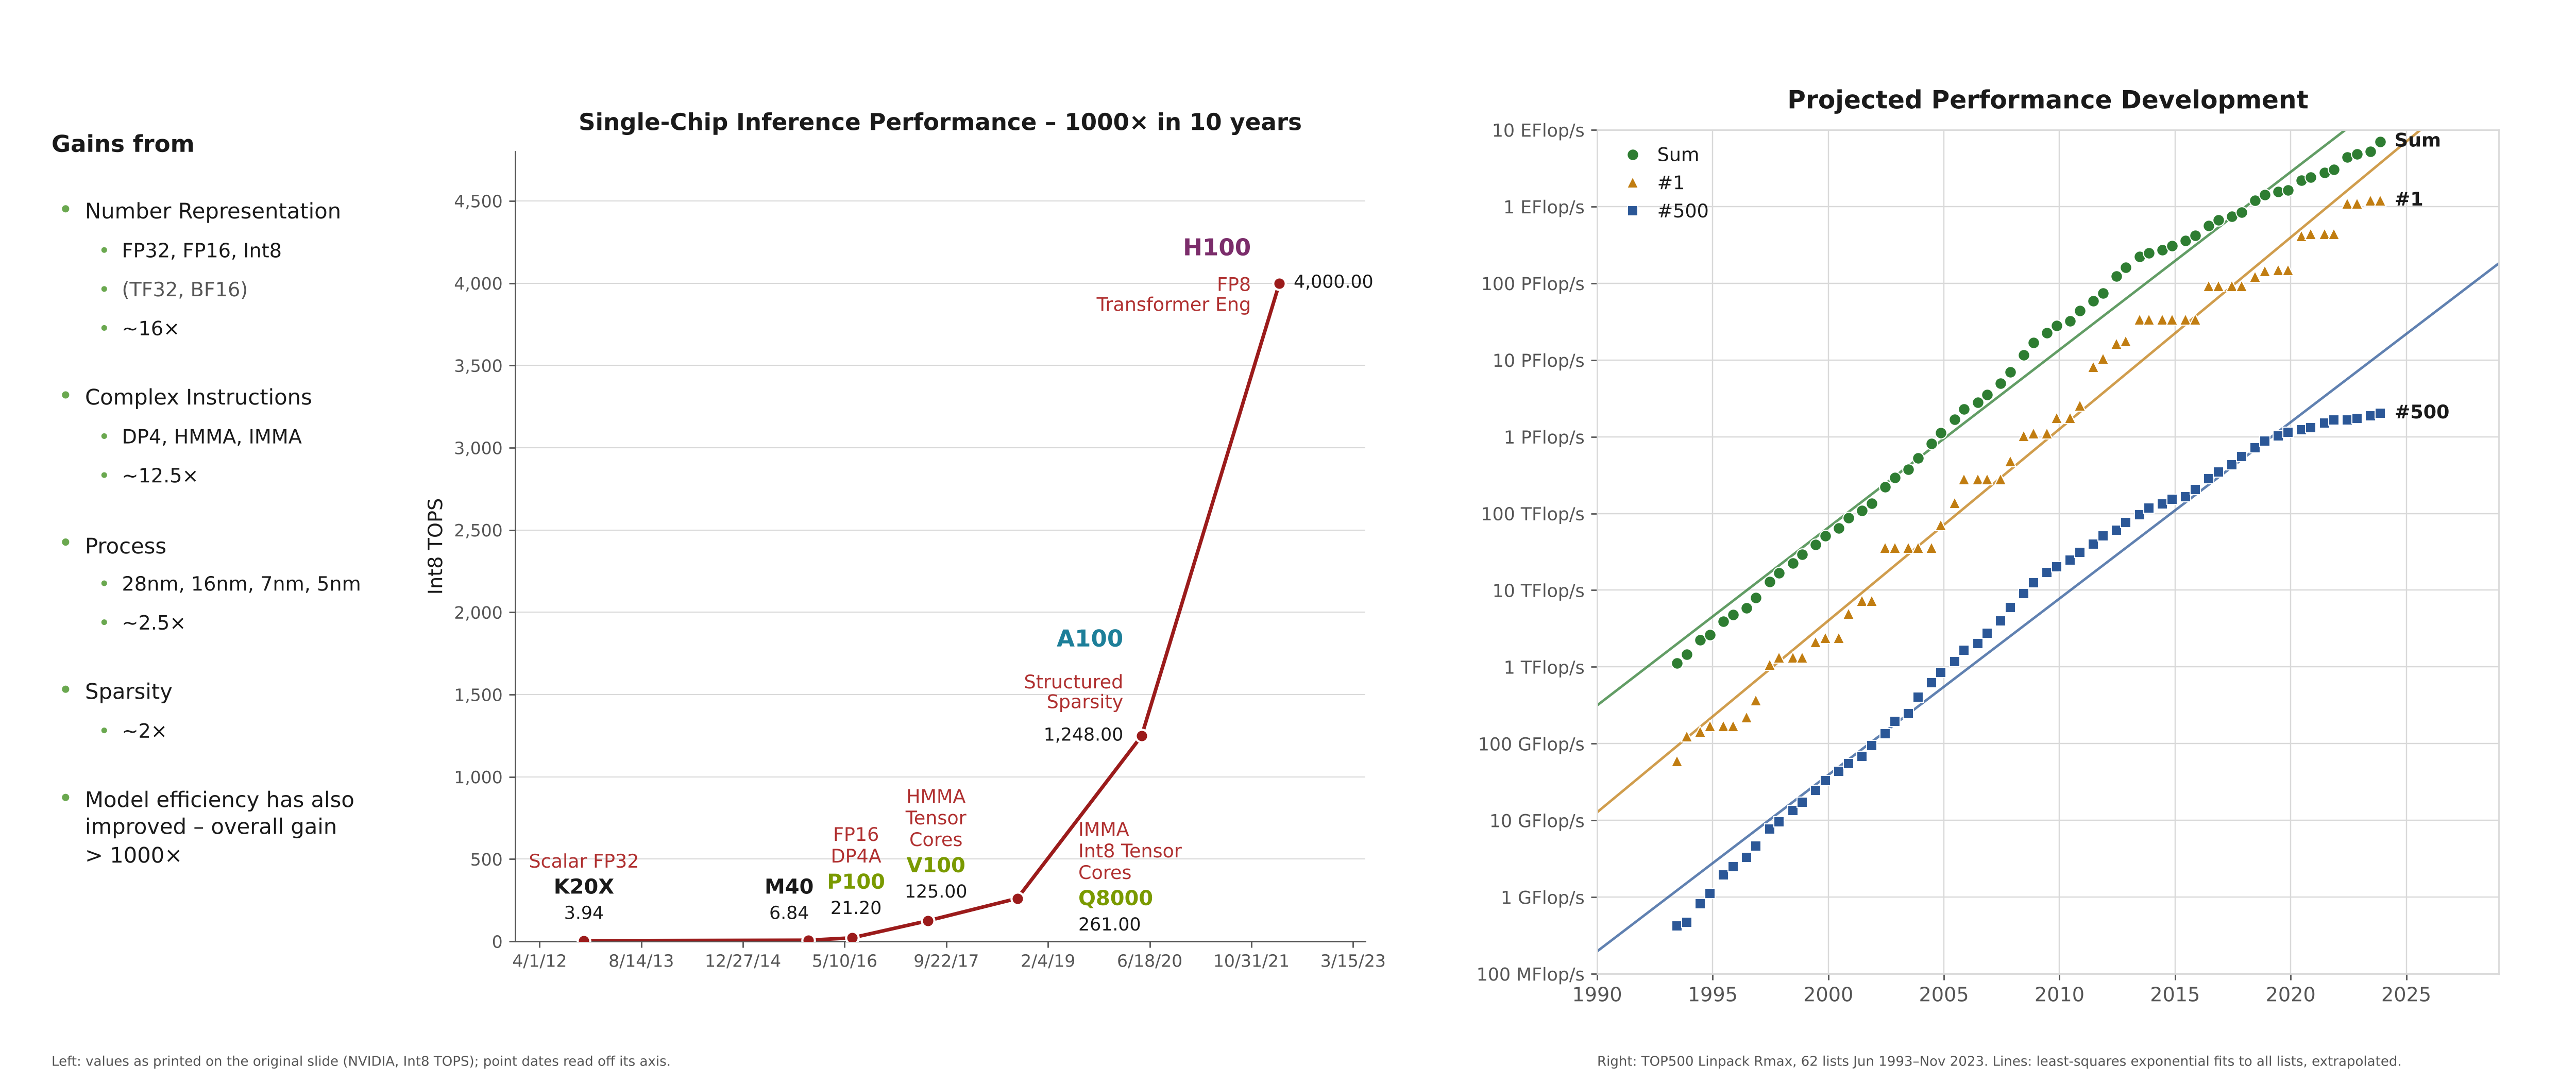
\includegraphics[width=1\linewidth]{combined.png}
\end{figure}

There are limits to single-GPU scaling.

\begin{center}
    The world's fastest supercomputers have \textit{exaflops} of compute.
\end{center}

\subsubsection*{Important detail : all-reduce vs reduce-scatter-gather}

Reduces can be implemented as two steps:

\begin{equation*}
    \text{All-reduce} = \text{Reduce-scatter} + \text{All-gather}.
\end{equation*}

Importantly, in the bandwidth-limited regime, this is the best you can do.

\subsubsection*{Limit to GPU scaling - memory}

Models are getting really big ..

\begin{figure}[hpbt]
    \centering
    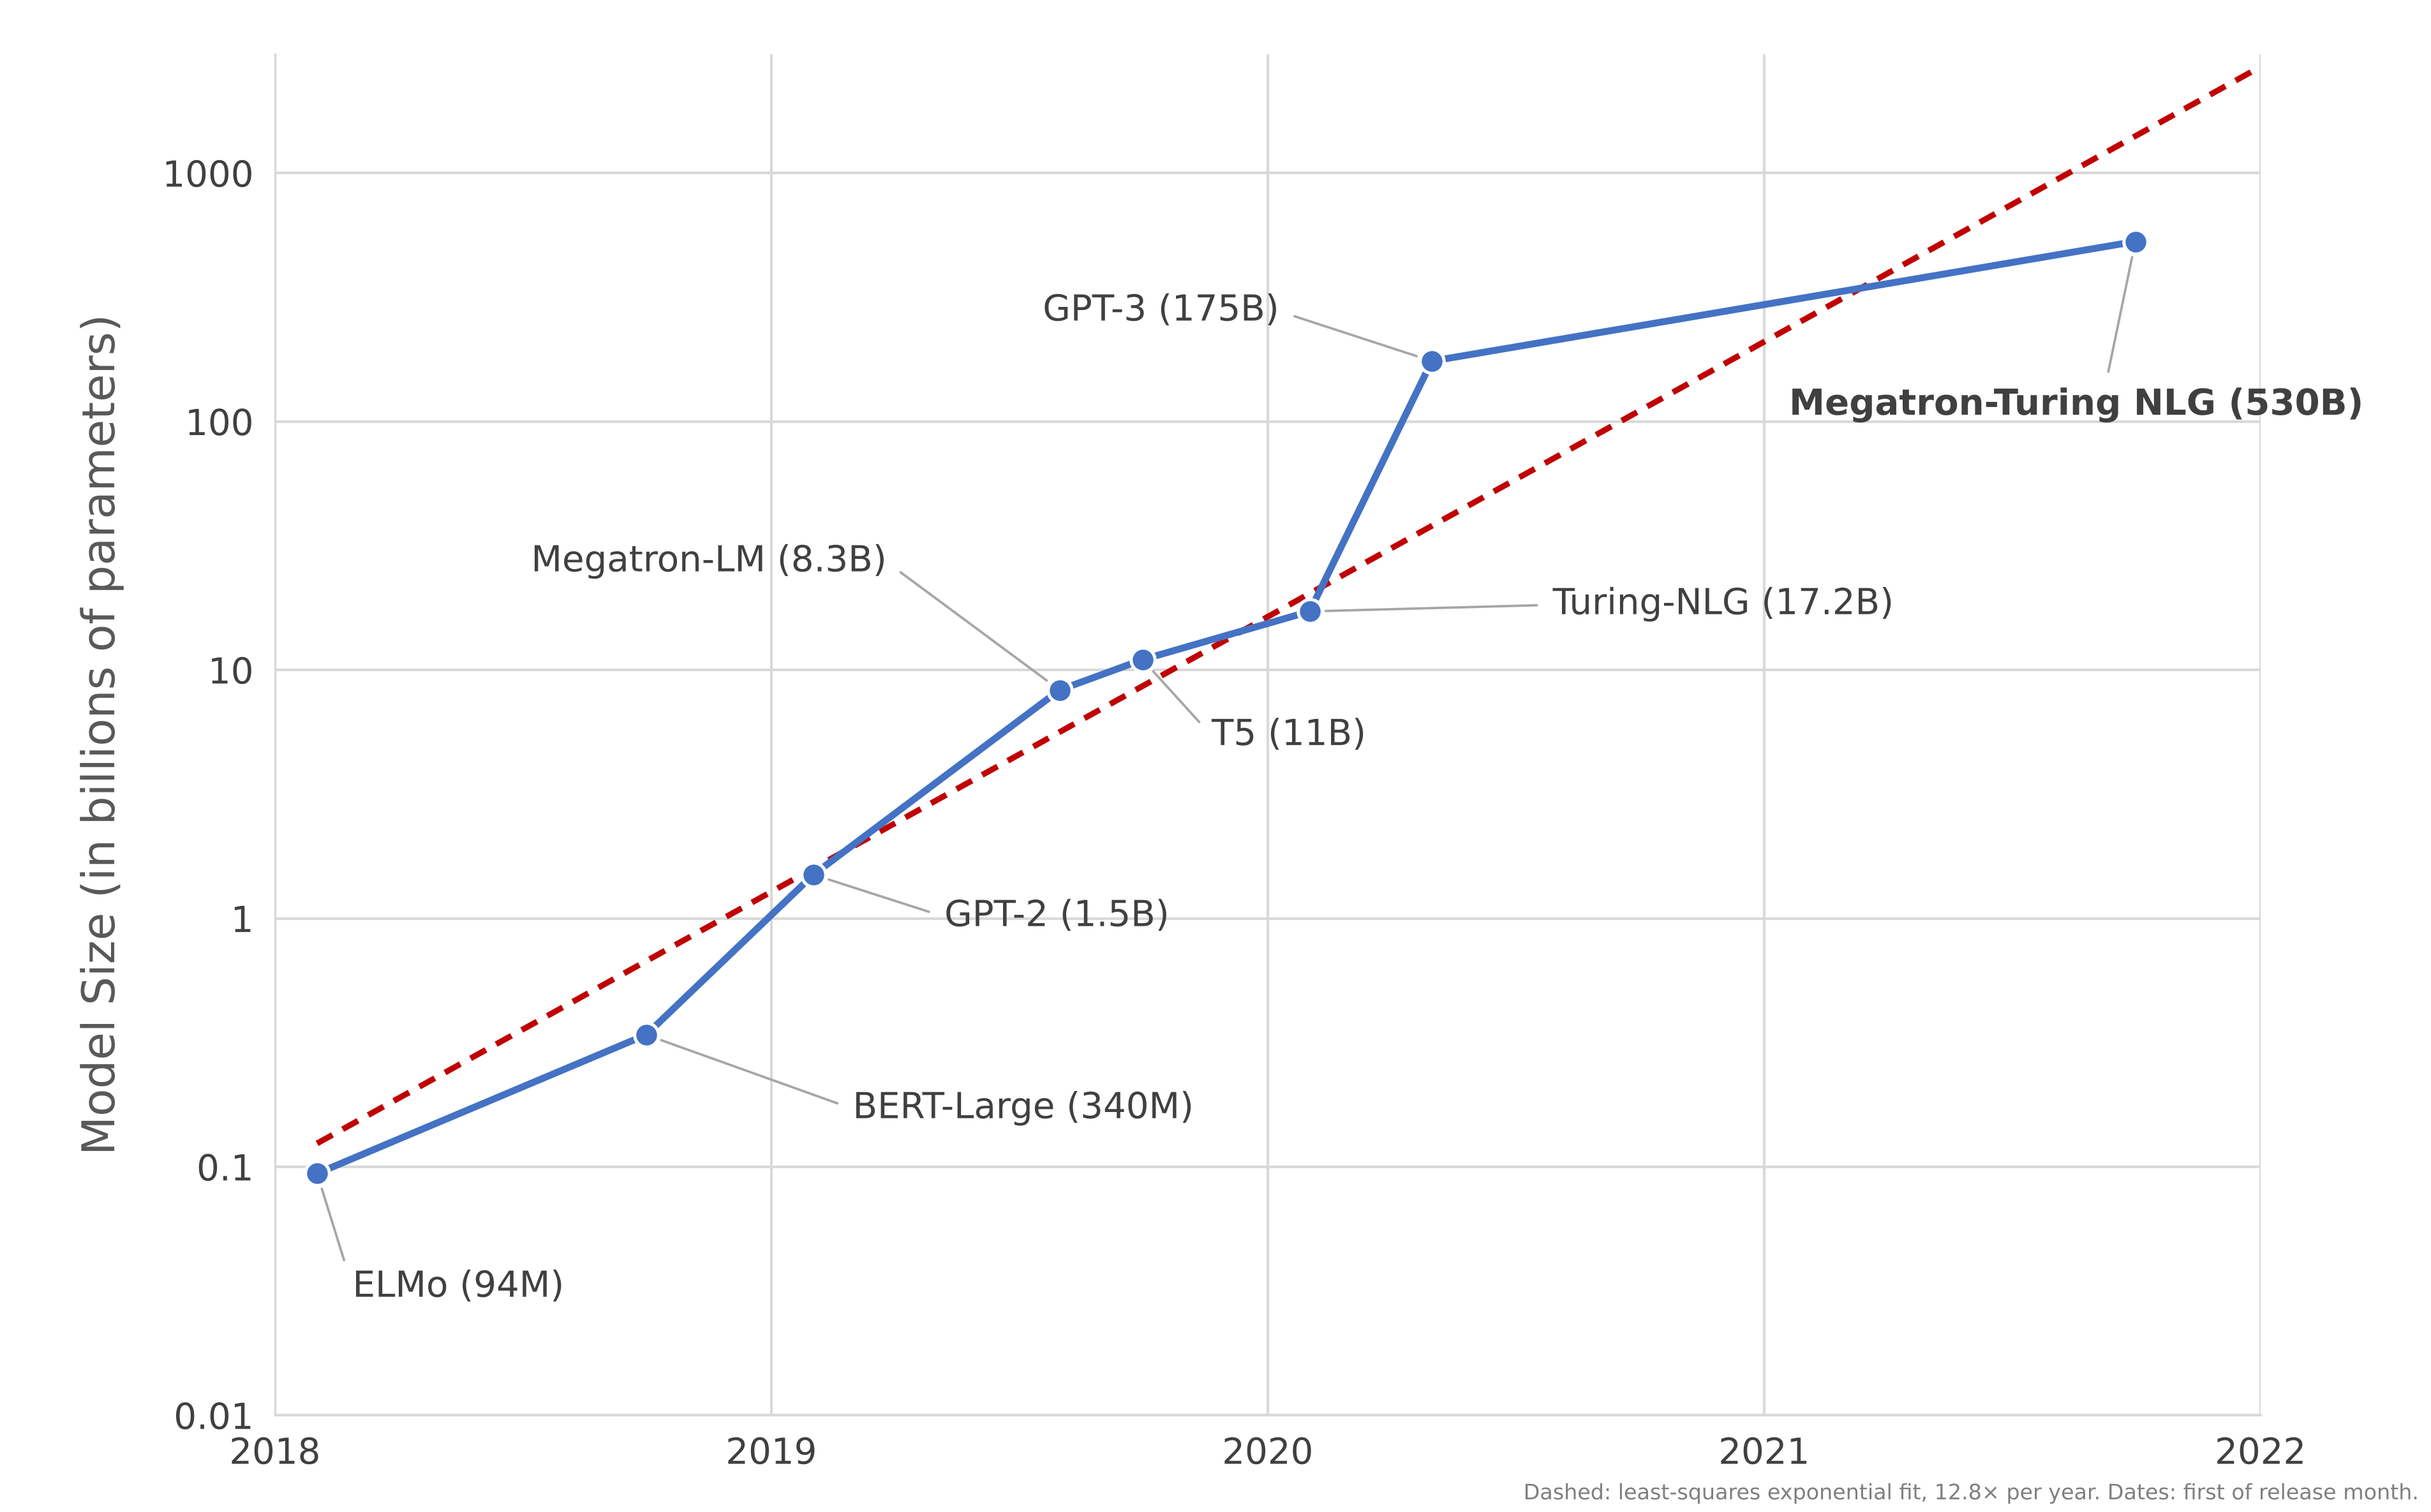
\includegraphics[width=1\linewidth]{model_size.png}
\end{figure}

\begin{center}
    A single GPU can't fit most of these large models!
\end{center}

\subsubsection*{GPUs vs TPUs - design differences at the communication level}

\begin{itemize}
    \item \textbf{GPU networking} \(=\) all-to-all (up to 256).
    \item \textbf{TPU networking} \(=\) toroidal mesh.
\end{itemize}

\subsubsection*{What do we do? Multi-GPU, multi-machine parallelism}

Intra-node parallelism (high-speed). \hfill Inter-node parallelism (slow-speed).

\begin{figure}[H]
    \centering
    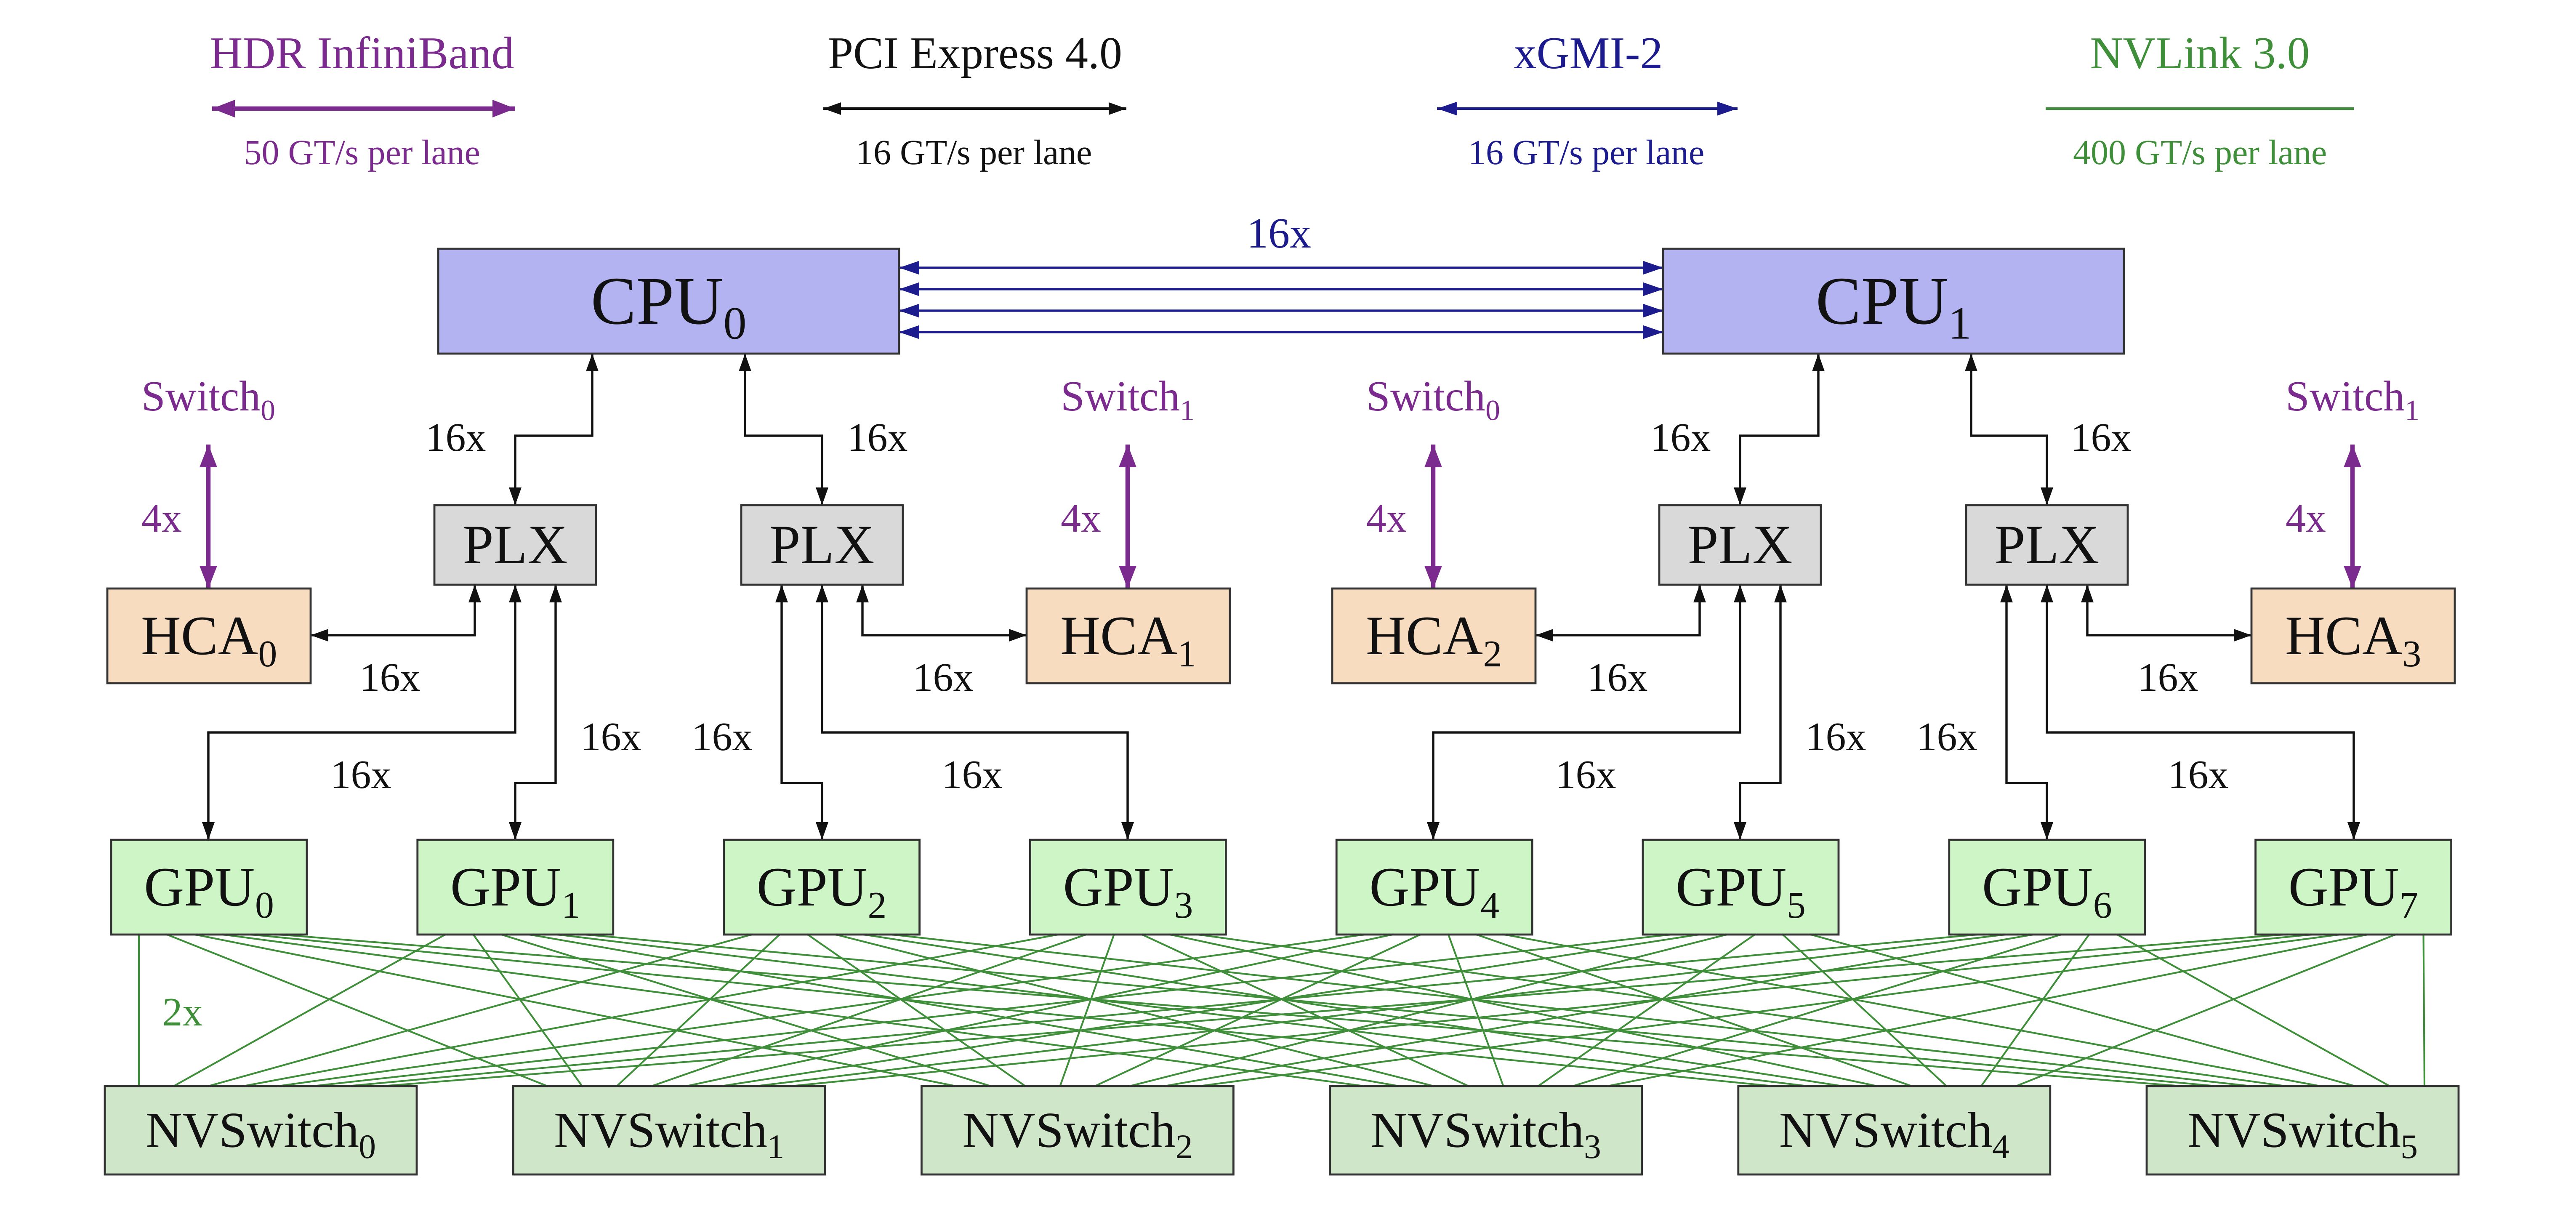
\includegraphics[width=1\linewidth]{dgx_a100_topology.png}
\end{figure}

\begin{center}
    Split up compute and memory requirements across GPUs and machines.
\end{center}

\subsubsection*{Why tree? Why mesh?}

\begin{center}
    Pro tree / A2A - Better for less structured communications (expert parallel).
\end{center}

\begin{center}
    Pro mesh - Cheaper to operate, can be made fast (and just do tensor parallel).
\end{center}

\subsubsection*{But then things changed .. TPU8i/t}

\begin{center}
    \textbf{TPU8i networking} - closer to tree-style topologies (maybe for MoEs?).
\end{center}

\begin{center}
    \textbf{TPU8t scale-out networking} - "Virgo" with switched networks.
\end{center}

\subsubsection*{Why not connect everything?}

\begin{center}
    \textbf{Key Capabilities} - Huawei Ascend 910C Cloud Matrix 384 \(=\) SRAM Everywhere!
\end{center}

\begin{center}
    New unit of compute - the datacenter.
\end{center}

\subsubsection*{What we want from multi-machine scaling:}

\begin{itemize}
    \item Linear compute scaling (model FLOPs scale linearly with num GPUs).
    \item Linear memory scaling (max model params scales with num GPUs) 
\end{itemize}

\subsection*{Standard LLM parallelization primitives}

How do we parallelize LLMs? 3 important ideas!

\begin{itemize}
    \item \textbf{Data parallelism} \begin{itemize}
        \item Naive data parallel 
        \item ZeRO levels 1-3
    \end{itemize}
    \item \textbf{Model parallelism} \begin{itemize}
        \item Pipeline parallel
        \item Tensor parallel
    \end{itemize}
    \item \textbf{Activation parallelism} \begin{itemize}
        \item Sequence parallelism
        \item Context parallelism
    \end{itemize}
\end{itemize}

\subsection*{Naive data parallelism}

\textbf{Starting point} - imagine we are doing naive SGD
\[
    \theta_{t + 1} = \theta_{t} - \eta \sum_{i = 1}^B \nabla f(x_i)
\]

\textbf{Naive parallelism}: split the elements of \(B\) sized batch across \(M\) machines and exchange gradients to synchronize. 

\begin{question}
    How does this do?
\end{question}

\begin{itemize}
    \item Compute scaling - each GPU gets \(B\)/\(M\) examples.
    \item Communication overhead - transmits 2\(\times\) \# params every batch. OK if batches are big.
    \item Memory scaling - every GPU needs \# params at least.
\end{itemize}

\subsubsection*{What's wrong with naive data parallel?}

\begin{center}
    Memory seems like it'd be a problem - we copy the model parameters to each GPU. Let's take a closer look ..
\end{center}

\begin{claim}
    Our memory situation is actually \textit{terrible}.
\end{claim}

Depending on our precision ..

\begin{center}
    \textbf{We need 5 copies of weights and 16 bytes per param!}
\end{center}

\begin{itemize}
    \item 2 bytes for FP/BF16 model parameters
    \item 2 bytes for FP/BF16 gradients
    \item 4 bytes for FP32 master weights (the thing you accumulate into in SGD)
    \item 4 (or 2) bytes for FP32/BF16 Adam first moment estimates
    \item 4 (or 2) bytes for FP32/BF16 Adam second moment estimates
\end{itemize}

\subsection*{ZeRO - solving the memory overhead issue of DP}

\textbf{Core idea}: split up the expensive parts (state) and use the reduce-scatter equivalence. 

\begin{figure}[hpbt]
    \centering
    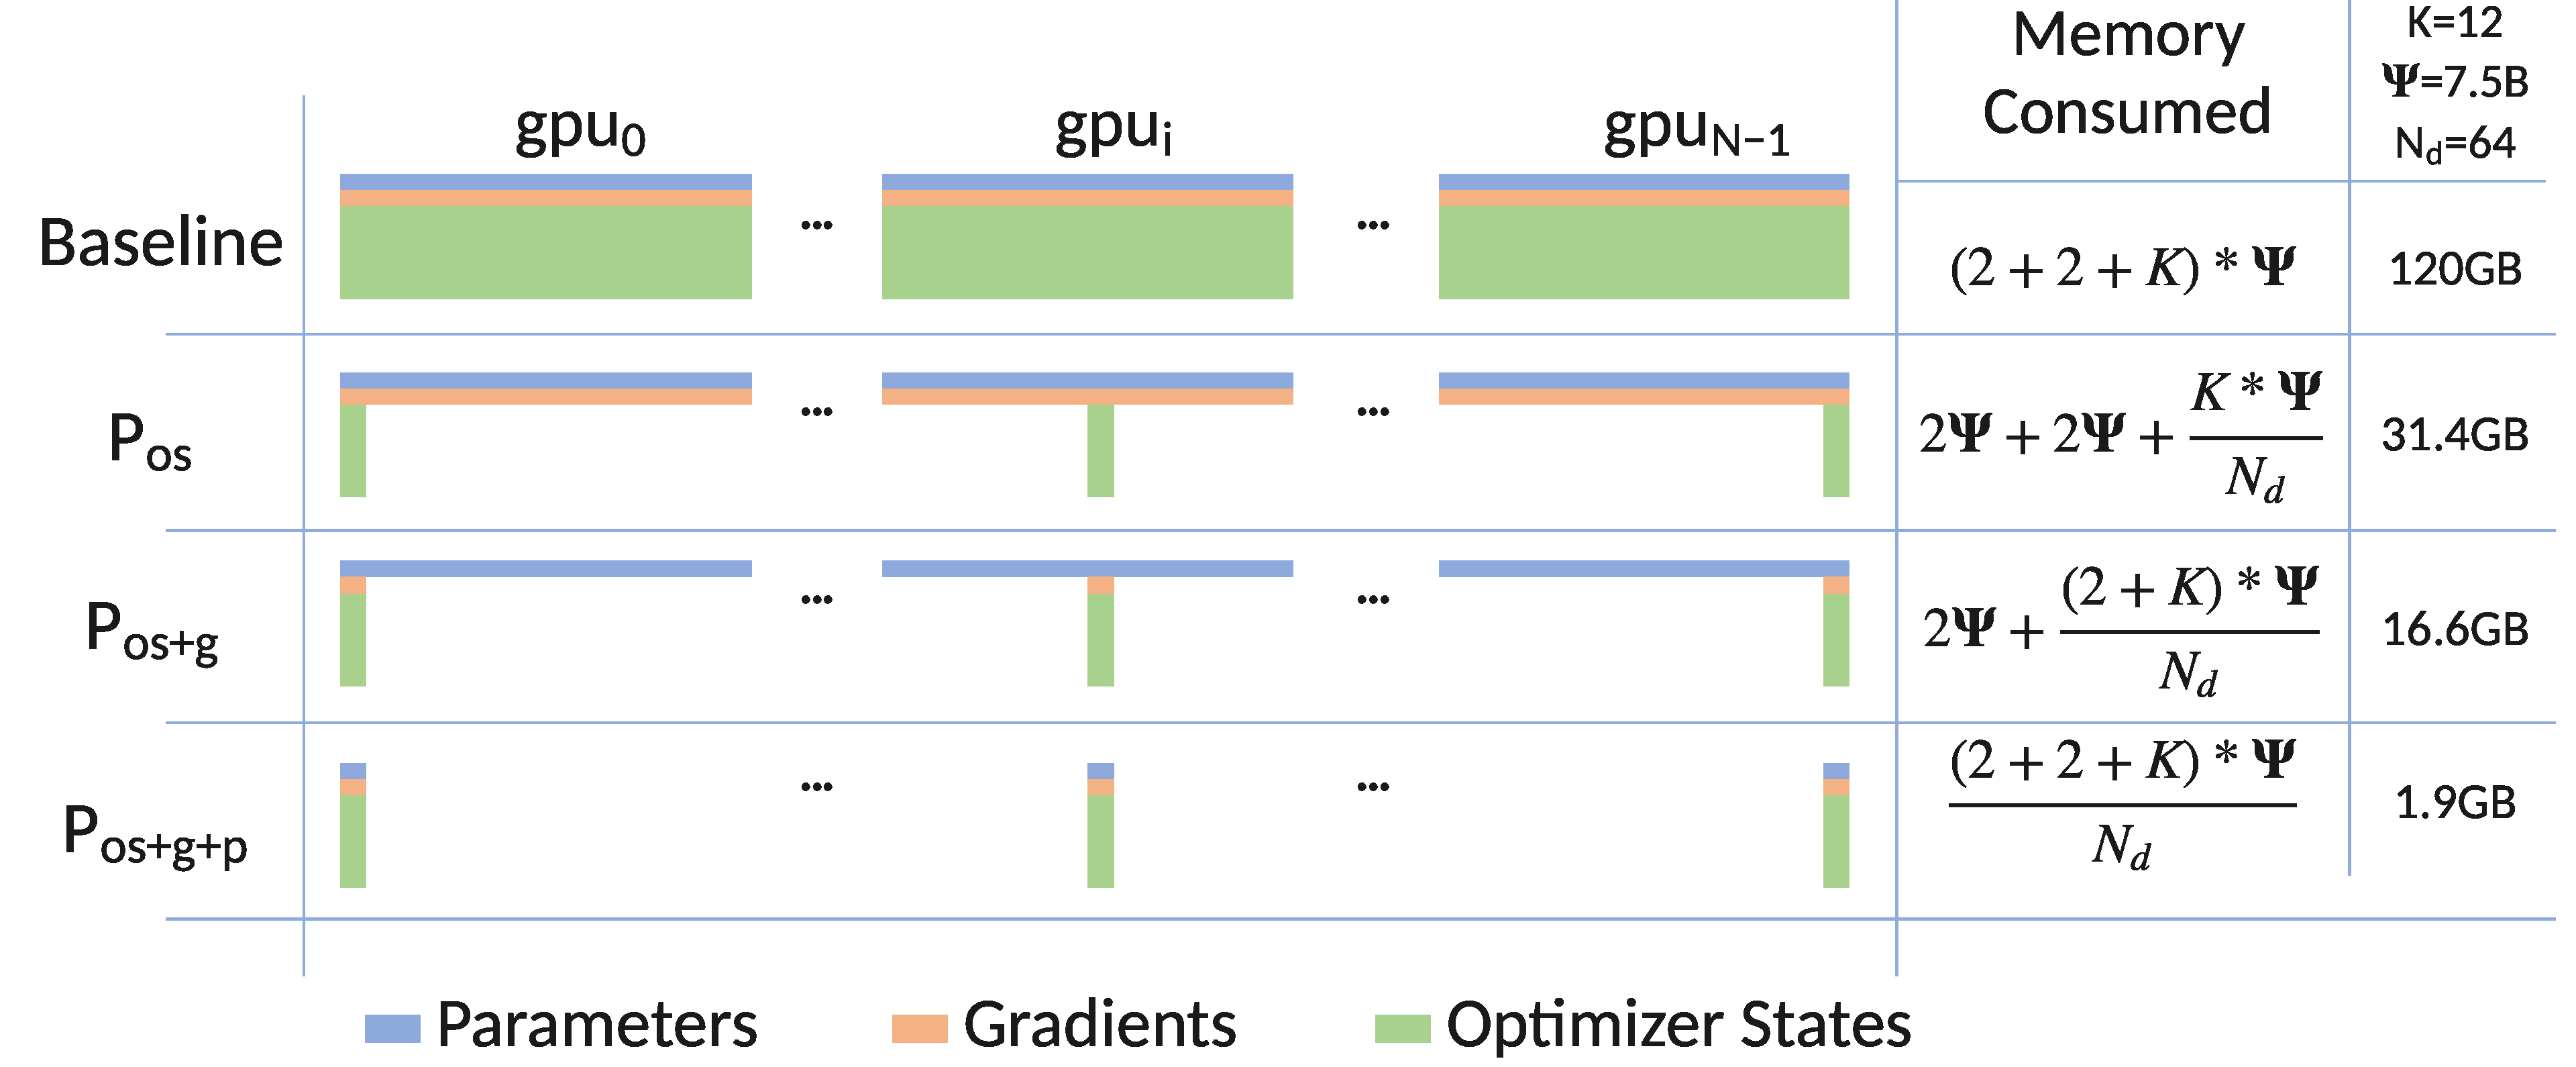
\includegraphics[width=1\linewidth]{zero_memory_partitioning.pdf}
\end{figure}

\subsubsection*{ZeRO stage 1. optimizer state sharding}

High level idea:
\begin{itemize}
    \item Split up the optimizer state (first \(+\) second gradients) across GPUs.
    \item Everyone has the parameters \(+\) gradients.
\end{itemize}

Each worker is responsible for updating a subset of params (corresponding to their slice).

\begin{center}
    \textbf{Step 1.} Everyone computes a full gradient on their subset of the batch.
\end{center}

\begin{center}
    \textbf{Step 2.} ReduceScatter the gradients - incur \# params communication cost.
\end{center}

\begin{center}
    \textbf{Step 3.} Each machine updates their param using their gradient \(+\) state.
\end{center}

\begin{center}
    \textbf{Step 4.} AllGather the parameters - incur \# params communication cost.
\end{center}

\begin{claim}
    ZeRO stage 1 is \textit{free} (in the bandwidth limited regime) memory wins.
\end{claim}

\subsubsection*{ZeRO stage 2. the simple extension to gradient sharding}

\begin{center}
    Emboldened by our success, let's shard even more stuff.
\end{center}

High level idea:
\begin{itemize}
    \item Also keep the gradients (pink slices) sharded across the machines.
    \item Use the same (rough) tricks as stage 1.
\end{itemize}

\textbf{Complexity} - we can never instaniate a full gradient vector, but each worker must compute a full gardient (since we're data parallel).

\begin{center}
    \textbf{Step 1.} After computing a layer's gradients, immediately reduce to send this to the right worker.
\end{center}

\begin{center}
    \textbf{Step 2.} Once the gradients are not needed in the backward graph, immediately free it.
\end{center}

\begin{center}
    \textbf{Step 3.} Each machine updates their param using their gradient \(+\) state.
\end{center}

\begin{center}
    \textbf{Step 4.} AllGather the parameters.
\end{center}

\subsubsection*{ZeRO stage 3 (aka FSDP) shard \textit{everything}}

\begin{center}
    We've gotten almost everything for free so far .. lets try to solve \textit{all} our memory issues.
\end{center}

High level idea:
\begin{itemize}
    \item Shard everything - incl parameters!
    \item Use the same "incremental computation / communication" ideas.
    \item Send and request parameters on demand while stepping through the compute graph.
\end{itemize}

\begin{figure}[hpbt]
    \centering
    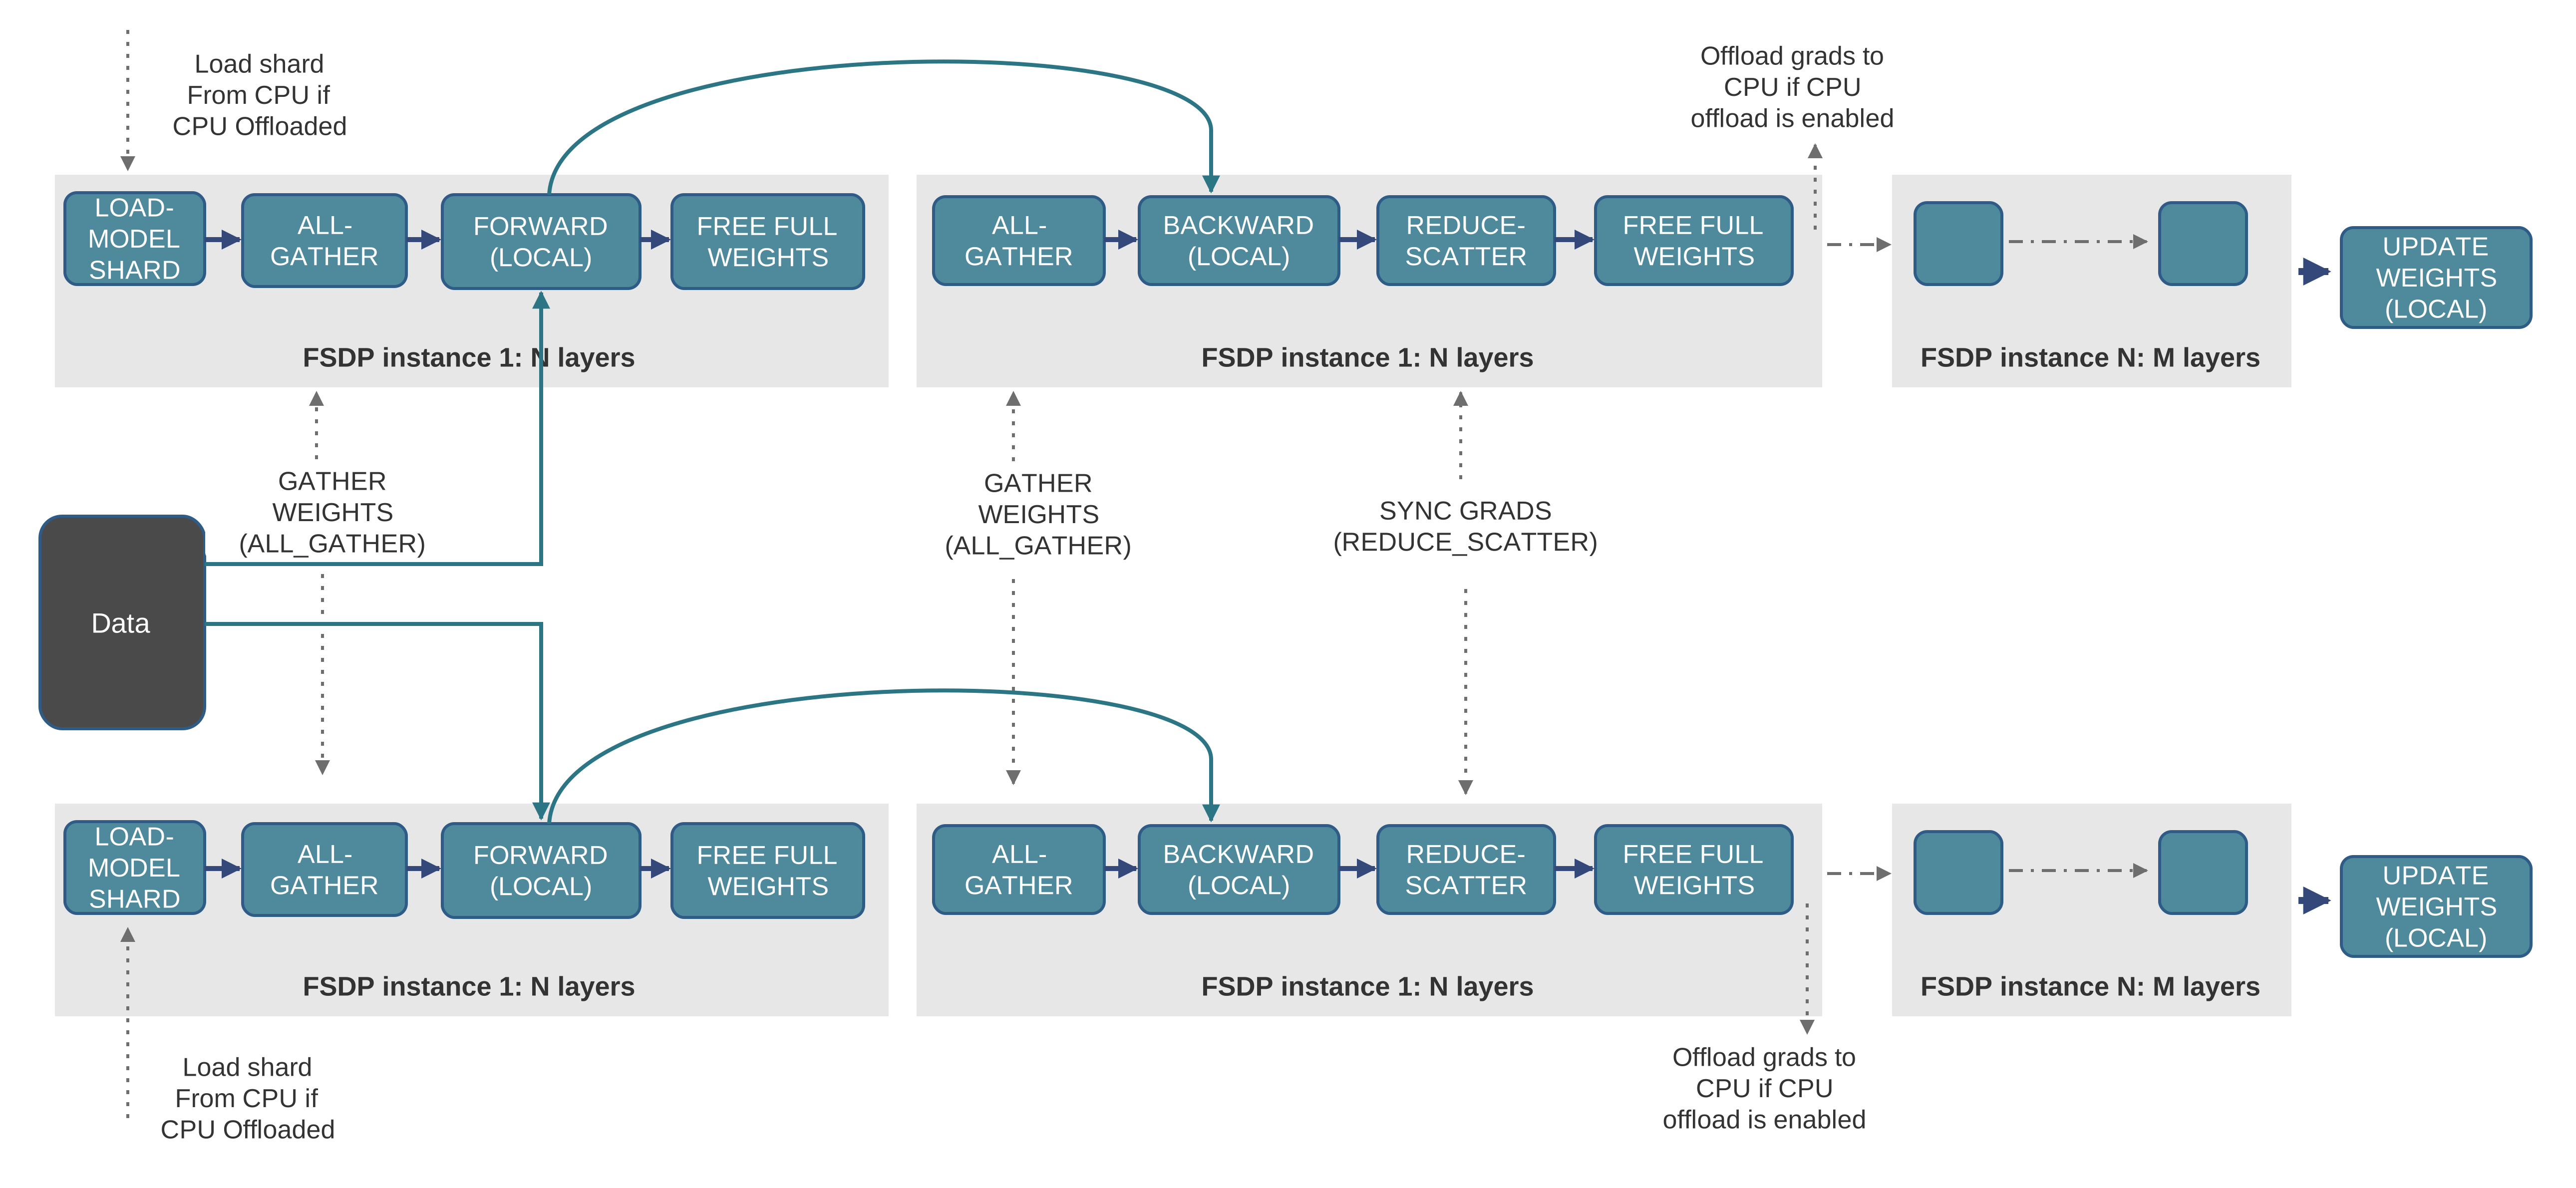
\includegraphics[width=0.75\linewidth]{fsdp_workflow.png}
\end{figure}

\begin{center}
    Communication cost - 2 AllGather (\# param), 1 ReduceScatter (\# param).
\end{center}

\textbf{Incremental computation / communication}
\begin{itemize}
    \item Parameters / gradients are requested / sent and then immediately freed. 
\end{itemize}

\textbf{Overlapping communication and computation}
\begin{itemize}
    \item The all-gathers happen all at once while forward happens, masking the communication cost.
\end{itemize}

\begin{figure}[hpbt]
    \centering
    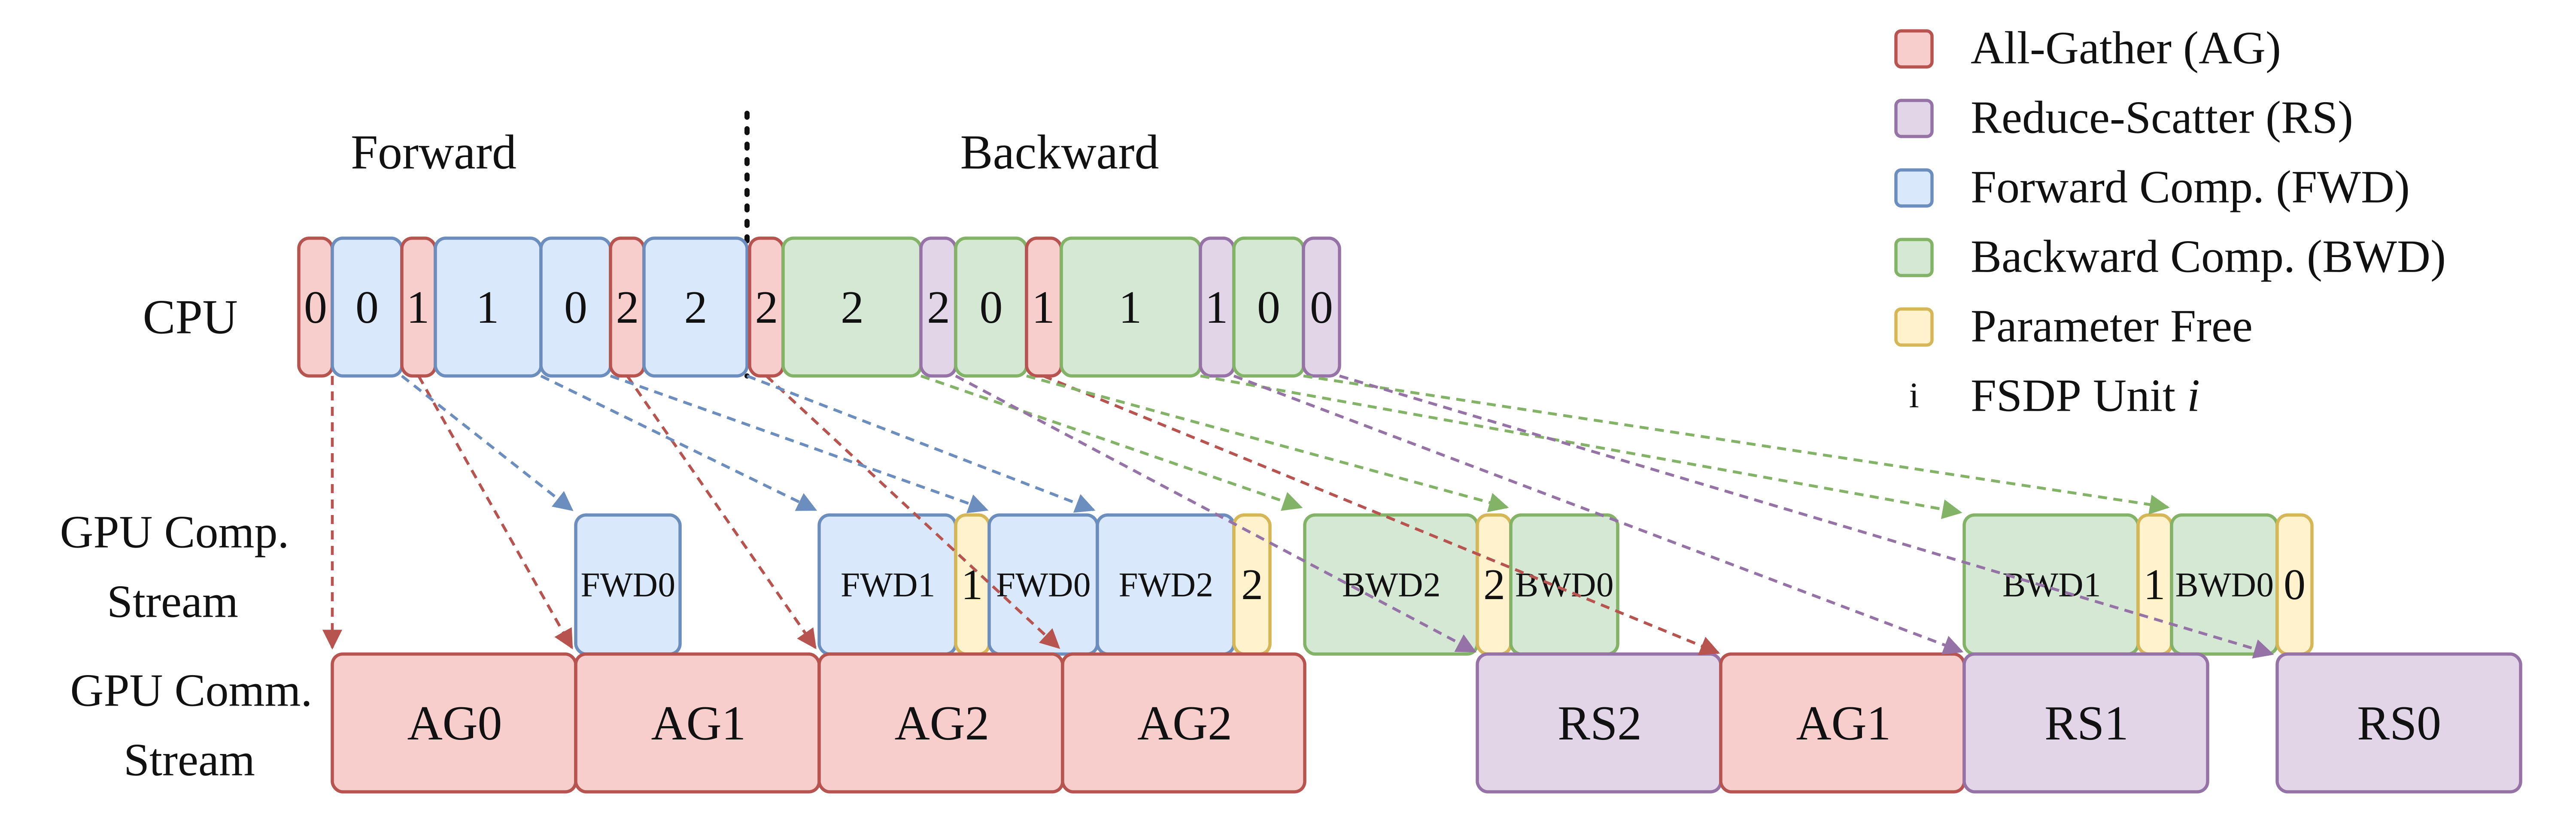
\includegraphics[width=1\linewidth]{fsdp_timeline.png}
\end{figure}

Distributed data parallel costs 2 \(*\) \# param communication.
\begin{itemize}
    \item \textbf{Zero stage 1} is 2 \(*\) \# param - it's free! - you might as well always do it.
    \item \textbf{Zero stage 2} is 2 \(*\) \# param - it's (almost) free (ignoring overhead).
    \item \textbf{Zero stage 3} is 3 \(*\) \# param - 1.5\(\times\) comm cost, but that's not bad (ignoring latency..)! 
\end{itemize}

This is also conceptually very simple - write a FSDP block wrapper.

\subsubsection*{Issue remain with data parallel - computing scaling}

\begin{center}
    With data parallel, \# machines \(<\) batch size (and near this, comm overhead is high).
\end{center}

\begin{center}
    And there's diminishing returns to batch sizes. 
\end{center}

\subsubsection*{Issue remain with data parallel - models don't fit}

\begin{center}
    \textbf{Zero stages 1 and 2} don't let you scale memory.
\end{center}

\begin{center}
    \textbf{Zero stage 3} is nice in principle, but \textit{does not reduce activation memory}.
\end{center}

Better ways to split up the model is needed ...

\subsection*{Beyond data parallel - model parallelism}

Scaling up in memory (without changing batch size) with model parallelism!

\begin{itemize}
    \item It splits up the parameters across GPUs (like ZeRO 3) ..
    \item But communicate activations (while ZeRO 3 sends params) ..
\end{itemize}

We cover 3 different types of parallelism!

\begin{enumerate}
    \item Pipeline parallelism
    \item Tensor parallelism (\(+\) sequential parallelism)
    \item Expert parallelism
\end{enumerate}

These correspond to three different ways of cutting up the model.

\subsubsection*{What's layer-wise parallel?}

\textbf{Layer-wide parallel} cuts up layers, assigns some subset to GPUs.

\begin{figure}[hpbt]
    \centering
    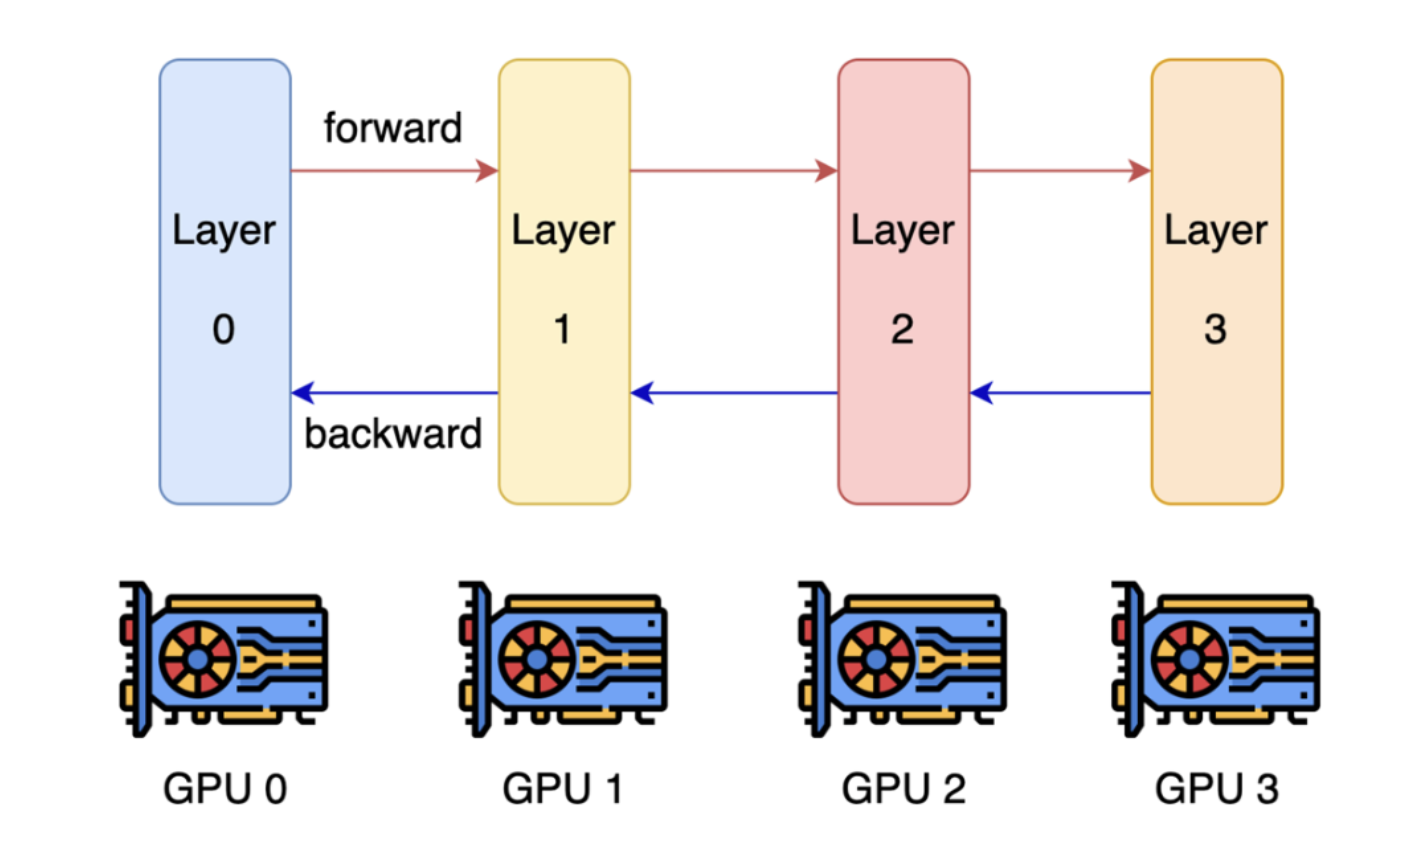
\includegraphics[width=1\linewidth]{layer-wise.png}
\end{figure}

\textbf{Activations and partial gradients} are passed back and forth.

\subsubsection*{What's wrong with layer-wise parallel?}

Utilization of layer-wise parallelism is \textit{terrible}..

\begin{center}
    With \(n\) GPUs, each GPU is active \(\frac{1}{n}\) of the time. 
\end{center}

\begin{figure}[hpbt]
    \centering
    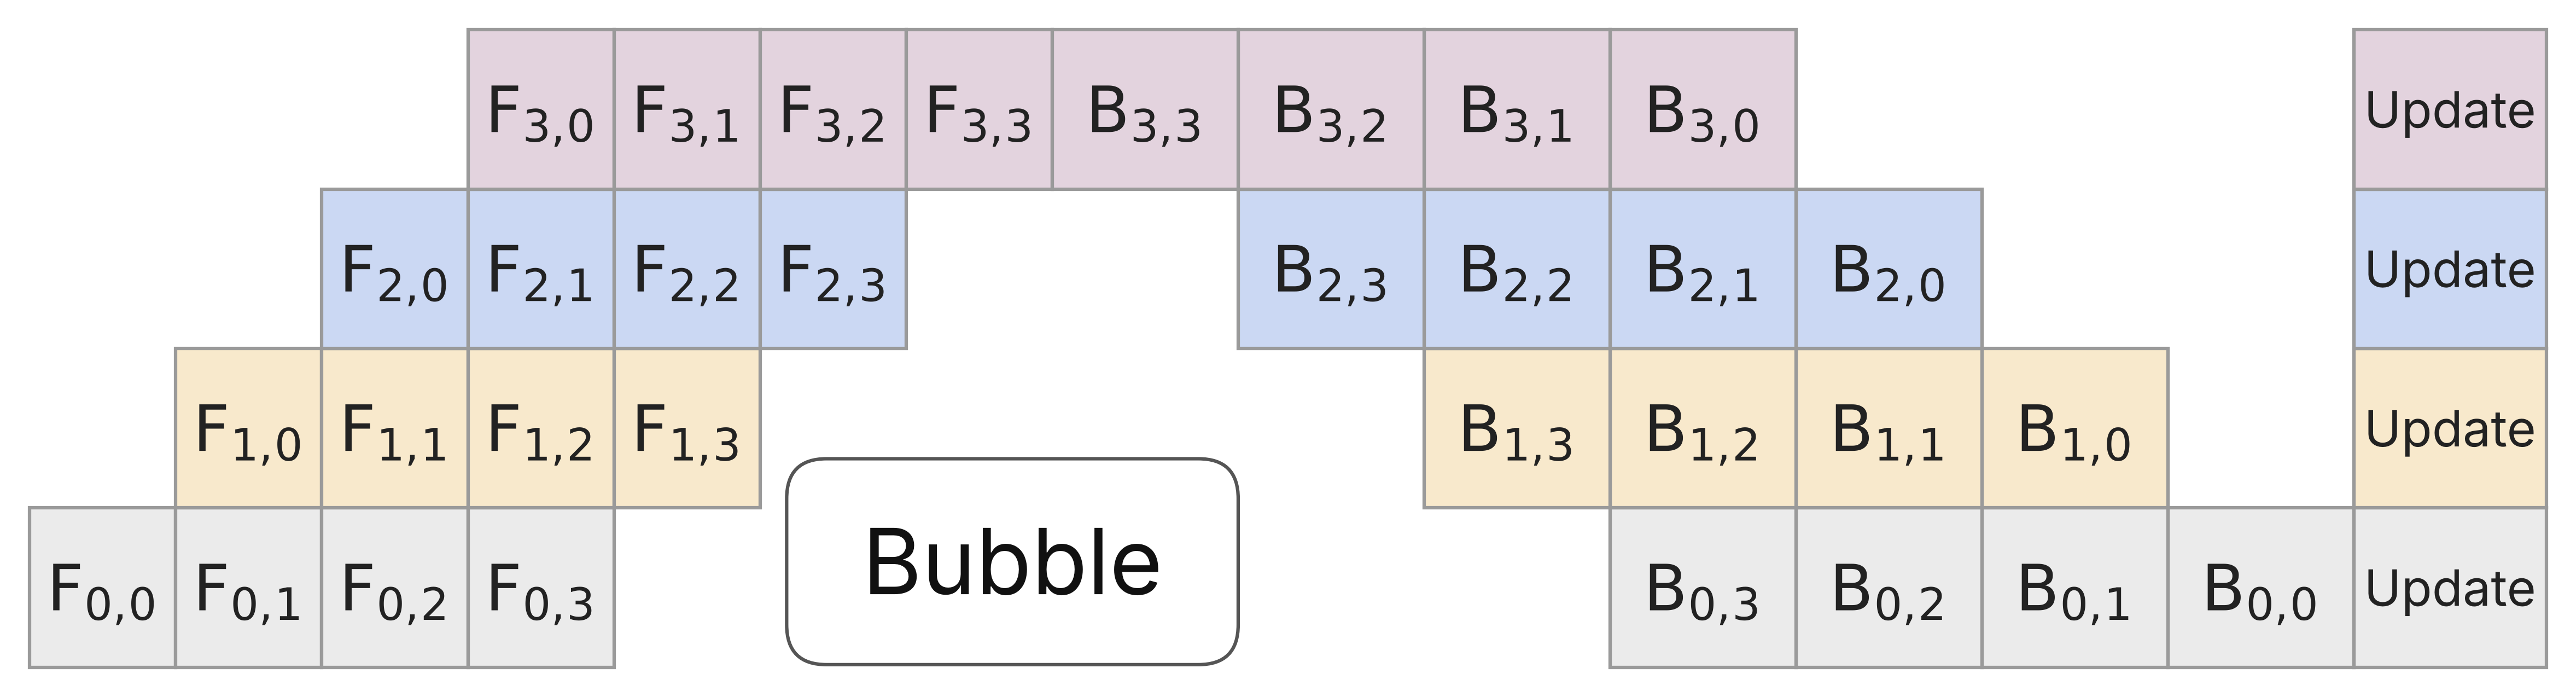
\includegraphics[width=1\linewidth]{gpipe_pipeline.png}
\end{figure}

\textbf{Solution: Pipeline-parallel.}

\begin{center}
    Process "micro-batches" (in this case, 4).
\end{center}

\begin{center}
    Send off the first microbatch and start computing the second.
\end{center}

The ratio of bubble time to useful compute compute is 
\[
    \frac{n_{\text{stage}} - 1}{n_{\text{micro}}}
\]
so we need a big batch size!

\subsubsection*{Why pipeline parallel?}

Pipelines seem terrible. Why do we do it?

\begin{enumerate}
    \item Pipelines save memory (compared to DDP)
    \item Pipelines can have good communication properties (compared to FDSP) - it depends only on activations (\(b \times s \times h\)) and is \textit{point to point} 
\end{enumerate}

Generally, we will use pipelines on slower network links (i.e. inter-node) as a way to get better memory-wise scaling.

\begin{itemize}
    \item Pipeline performance is highly dependent on batch size
    \item Batch sizes are key to hiding the buddle - otherwise pipeline rapidly degrades performance
    \item Trade communication  bandwidth for utilization
    \item Some more crazy pipeline patterns can improve utilization, but at the cost of bandwidth
\end{itemize}

\subsubsection*{"Zero bubble" pipelining}

Split up backwards into 2 parts

\begin{enumerate}
    \item Backpropagating activations (\(x, z\))
    \item Computing weight gradients (\(W\))
\end{enumerate}

\begin{claim}
    The second part can be done whenever.
\end{claim}

\begin{figure}[hpbt]
    \centering
    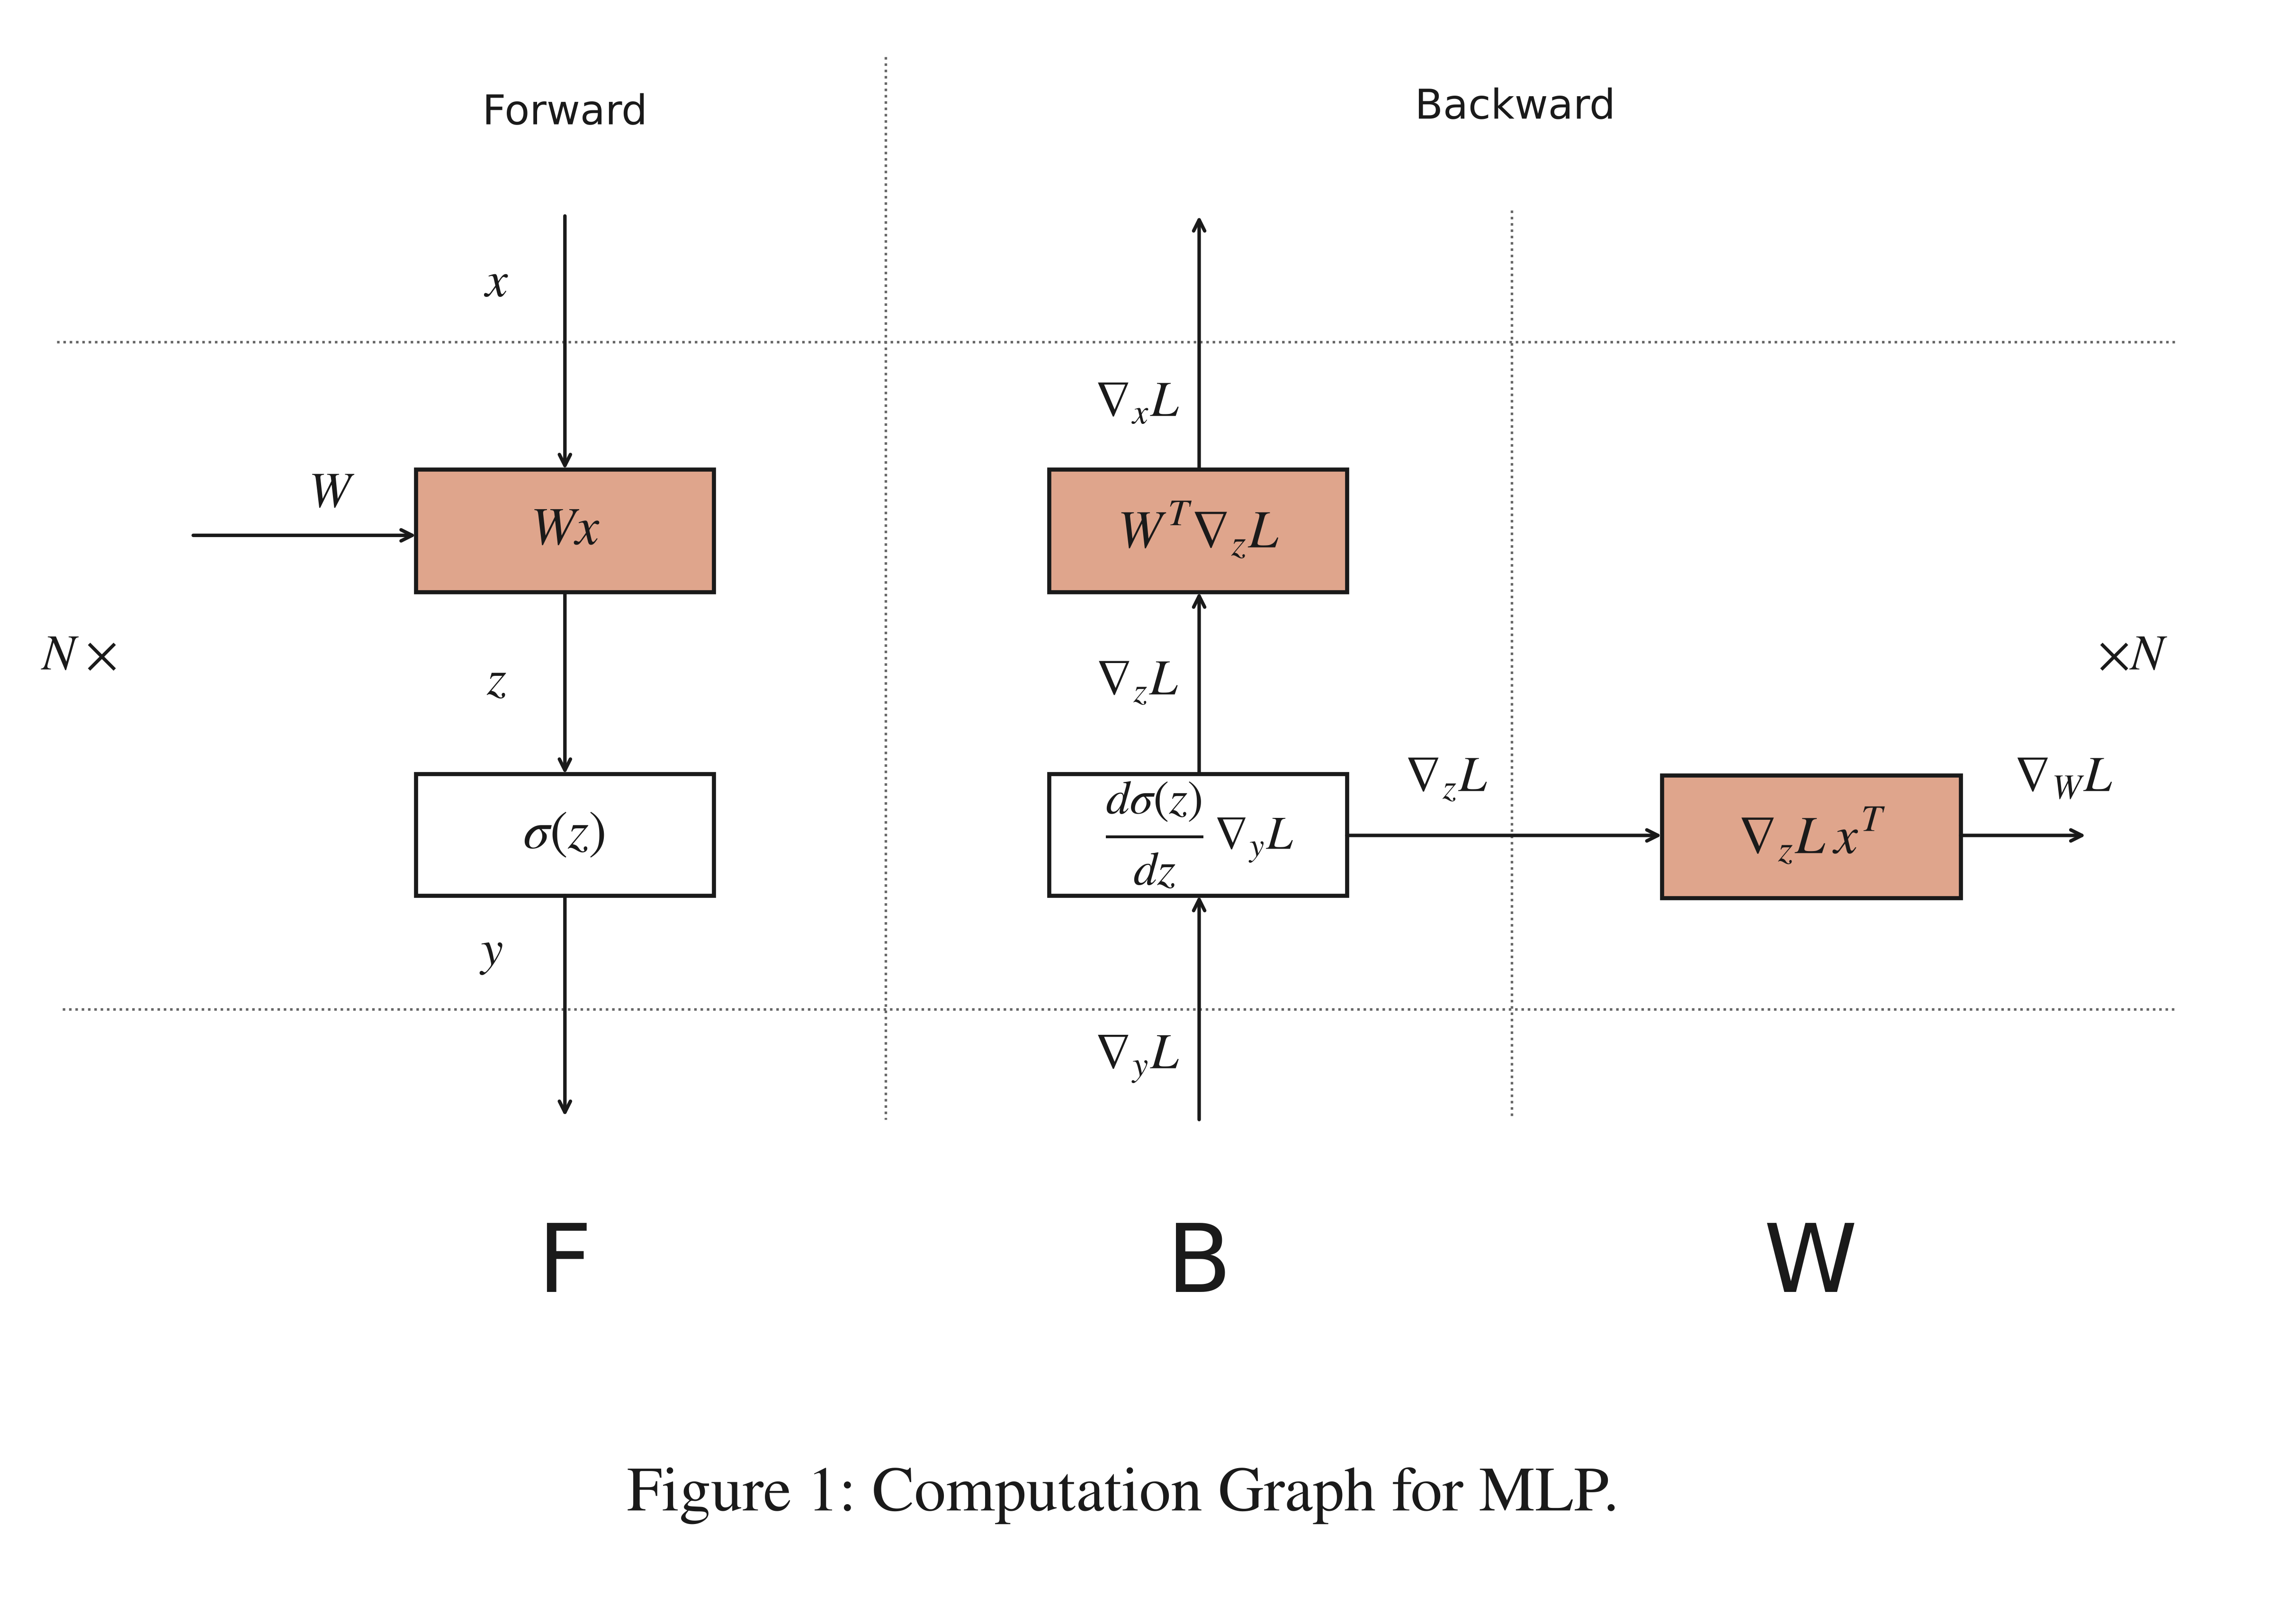
\includegraphics[width=1\linewidth]{mlp_computation_graph.png}
\end{figure}

\subsubsection*{Model parallel along the width axes}

\begin{question}
    Are there model parallel schemes with better utilization?
\end{question}

\begin{itemize}
    \item We can think of pipeline parallel as cutting up along depth. What about width?
    \item Simple matrix multiplication observation: decompose into submatrices, add partial sums.
\end{itemize}

\subsubsection*{Tensor parallel - GPUs have submatrices}

\begin{figure}[H]
    \centering
    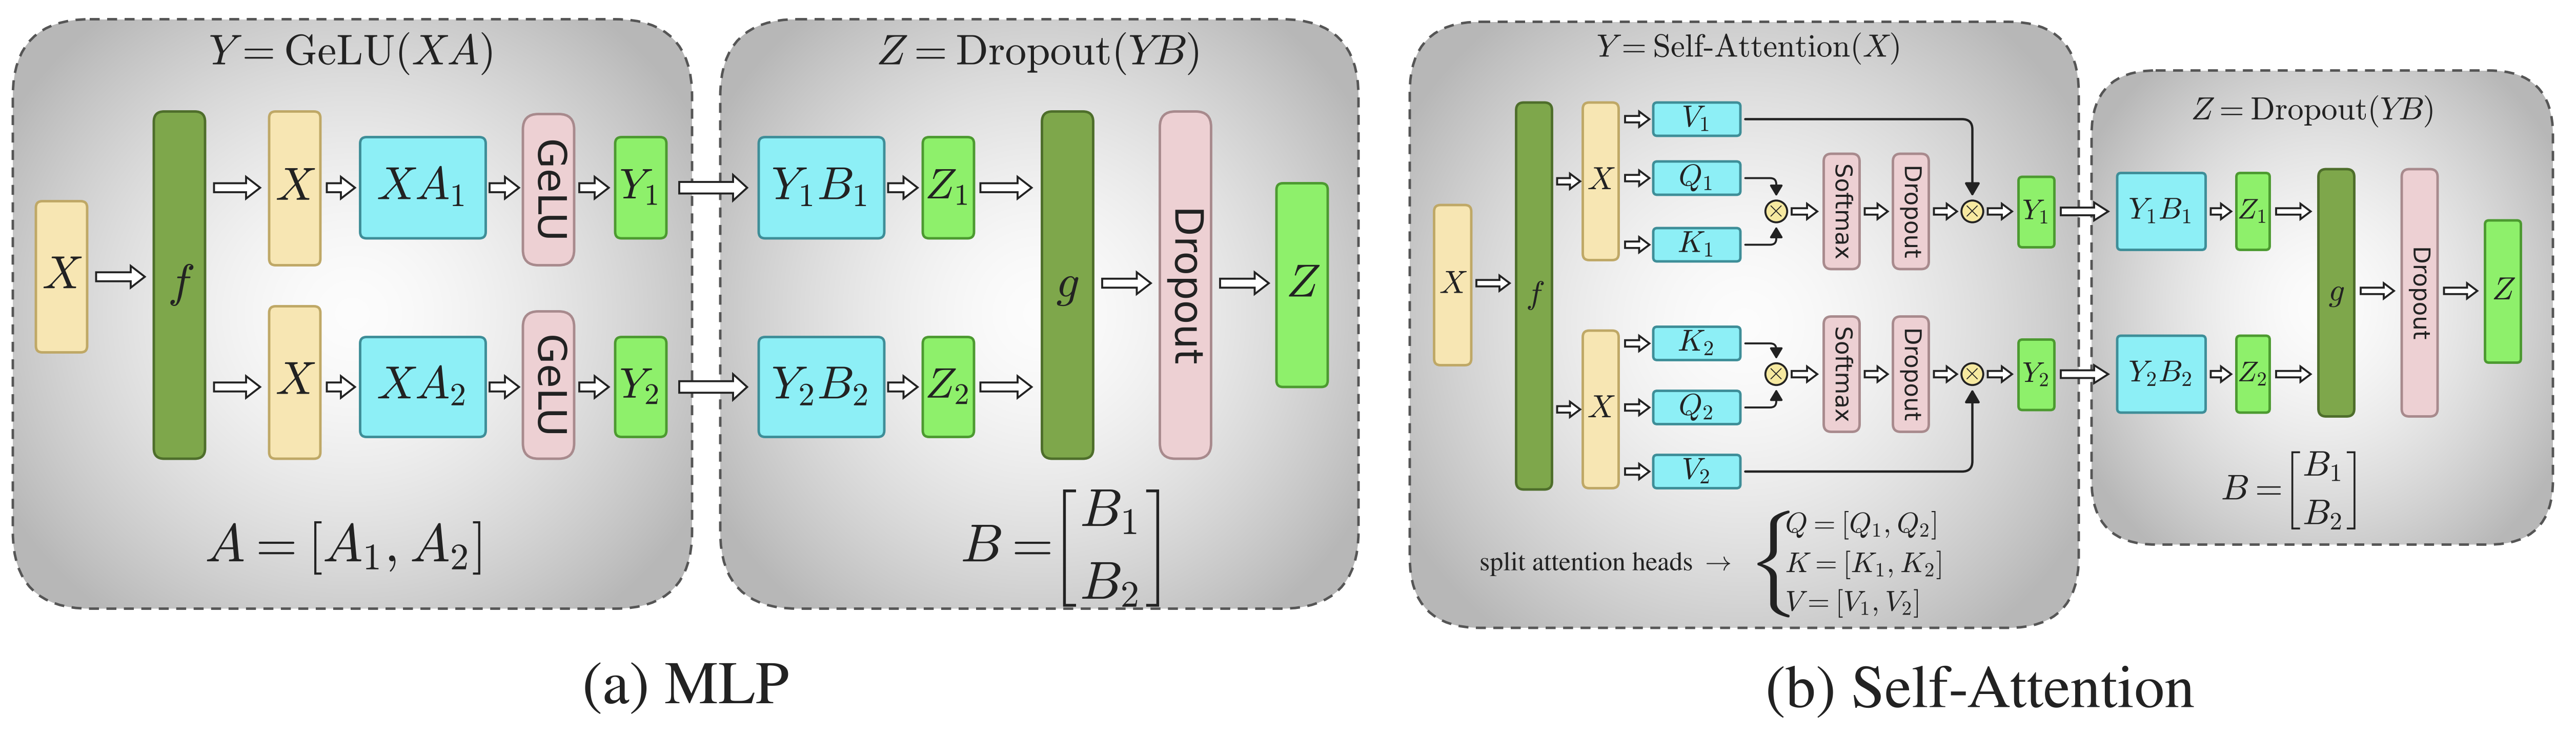
\includegraphics[width=1\linewidth]{megatron_tp.png}
\end{figure}

Assign columns (\(A1,A2\)) and rows (\(B1,B2\)) to separate GPUs.

\begin{itemize}
    \item In the forward pass, \(f\) is the identity and \(g\) is an all-reduce.
    \item In the backward pass, \(f\) is an all-reduce, \(g\) is the identity.
\end{itemize}

How do we split up in tensor parallel across a transformer block?

\begin{itemize}
    \item Columnwise - \(QKV\), up-projection
    \item Rowwise - Attention output, down-projection
    \item Replicated - norms, routers, etc
\end{itemize}

\subsubsection*{When do we tensor parallel?}

On GPUs, tensor parallel within a node (up to 8 GPUs) due to high speed interconnects.

\begin{center}
    How do things compare to pipeline parallel?
\end{center}

\textbf{Pros}

\begin{itemize}
    \item No bubble. If your network is fast enough, there's no waiting for others.
    \item Low-complexity. It is simple to "wrap" models without major infrastructure changes.
    \item Doesn't need large batch size to work well.
\end{itemize}

\textbf{Cons}

\begin{itemize}
    \item Much larger communication than pipeline parallel.
    \item Pipeline: \(bsh\) point-to-point communication per microbatch.
    \item Tensor: \(8bsh \left(\frac{n_{\text{devices}} - 1}{n_{\text{devices}}}\right)\) per layer and all-reduce communication.
\end{itemize}

\begin{center}
    Use tensor parallel whenever we have low-latency, high-bandwidth interconnects. 
\end{center}

\subsubsection*{A final complexity - memory is dynamic!}

Memory isn't just the static bits, but also activations! This can be very large!

\begin{itemize}
    \item Thus far, we have only really discussed parameter memory.
    \item Tensor and pipeline parallel can linearly reduce those .. \tectbf{but what about activations?}
\end{itemize}

\begin{center}
    What's the activation memory per layer?
\end{center}

\textbf{Starting point:} activation memory needed if storing everything.

\begin{equation*}
    \text{Activations memory per layer} = sbh\left(34 + 5\frac{as}{h}\right)
\end{equation*}

\begin{itemize}
    \item The \(5\frac{as}{h}\) term comes from the quadratic attention terms including dropout.
    \item As with flash attention, we can drop this term via recomputation.
\end{itemize}

\textbf{Next point:} activation memory under tensor parallel.

\begin{equation*}
    \text{Activations memory per layer} = sbh\left(10 + \frac{24}{t} + 5\frac{as}{ht}\right)
\end{equation*}

\begin{itemize}
    \item Tensor parallel splits the matrix multiples in attention \(+\) MLP.
    \item The remaining 10 term is for the LayerNorm (\(4sbh\)), Dropout (\(2sbh\)), and inputs to attention and MLP (\(4sbh\)).
    \item These terms alone will continue to grow with size.
\end{itemize}

\subsubsection*{Making memory truly linear - sequence parallel}

\begin{figure}[hpbt]
    \centering
    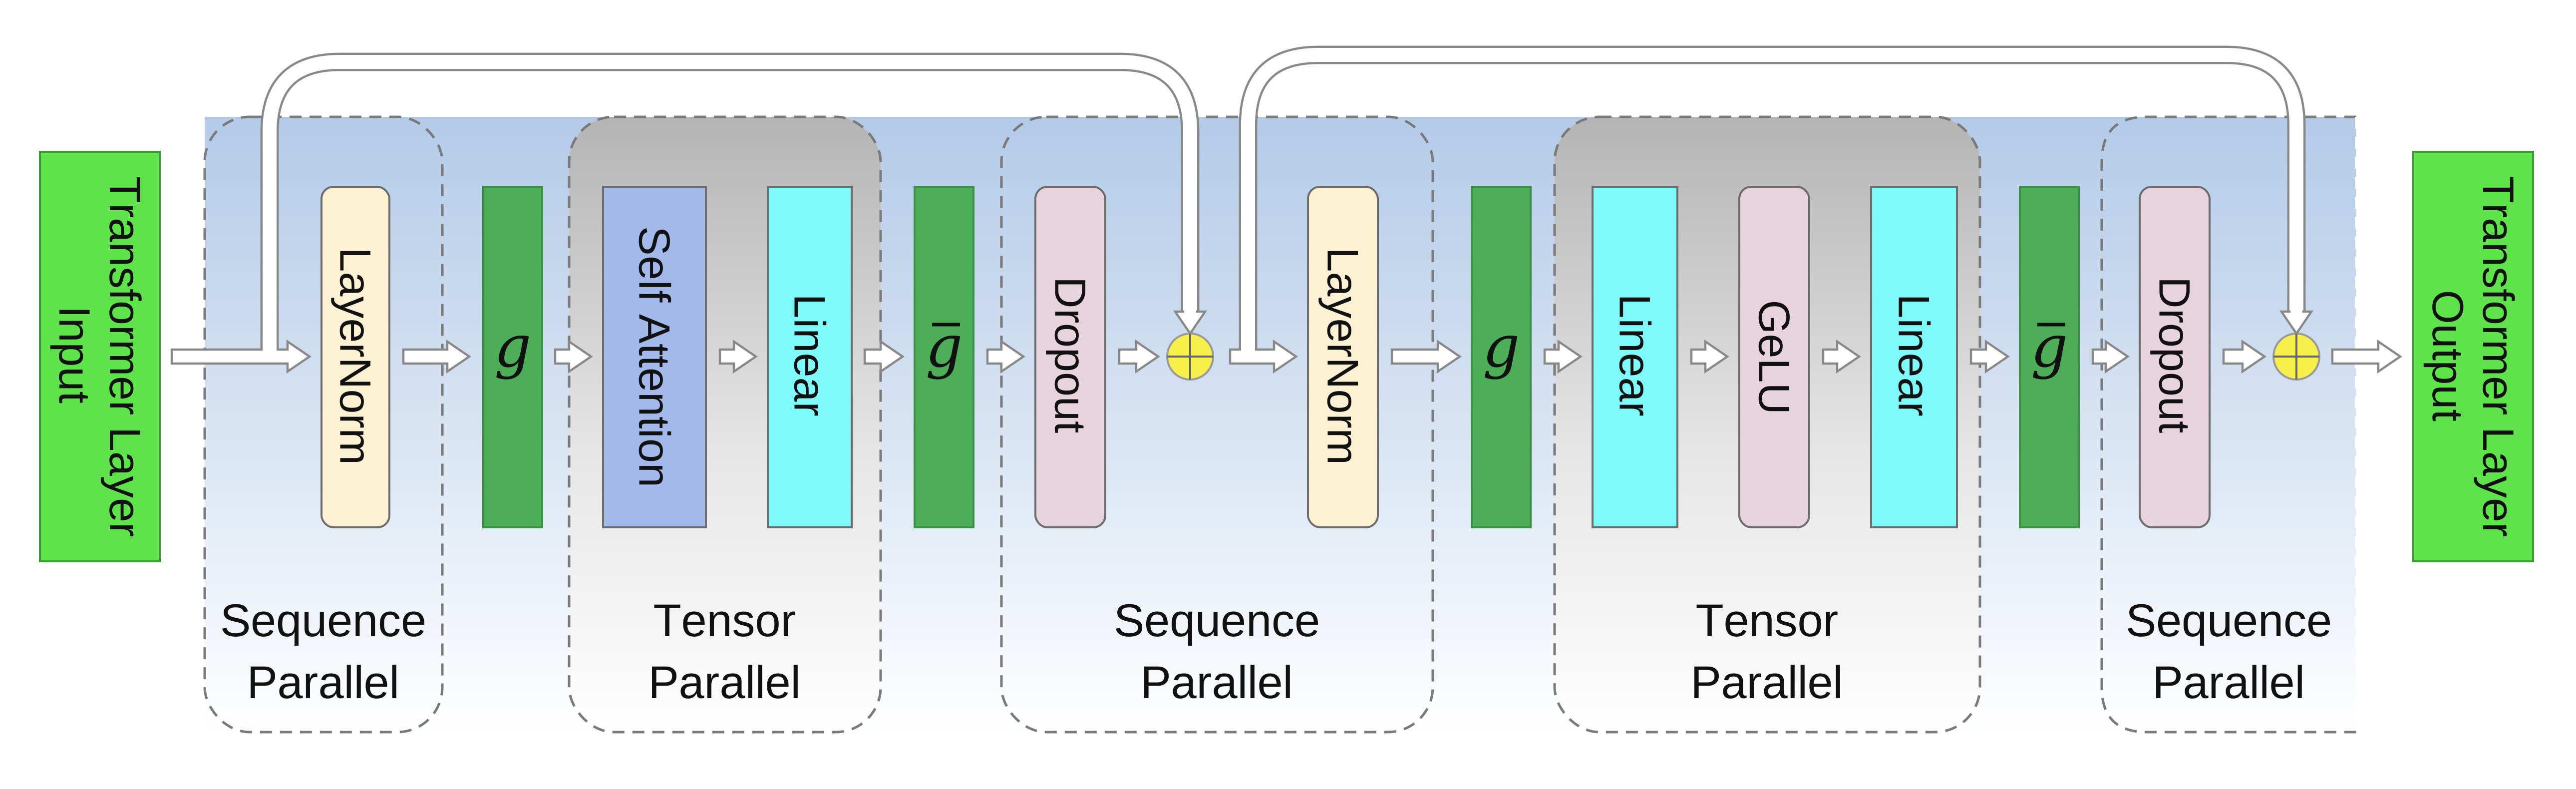
\includegraphics[width=1\linewidth]{sp_tp_layer.png}
\end{figure}

\textbf{Observation:} all the \(10sbh\) terms are pointwise operations over the sequence .. so split up the layer norm/dropout layers along the sequence axis.

\begin{itemize}
    \item In the forward pass, '\(g\)' is an all-gather and '\(\overline{g}\)' is reduce-scatter.
    \item In the backward pass, '\(g\)' and '\(\overline{g}\)' are reversed.
\end{itemize}

\begin{center}
    Making activation memory fully scale with more machines.
\end{center}

\subsubsection*{Expert parallelism}

Instead of splitting up the matmul, split up the expertd and route activations.

\begin{figure}[hpbt]
    \centering
    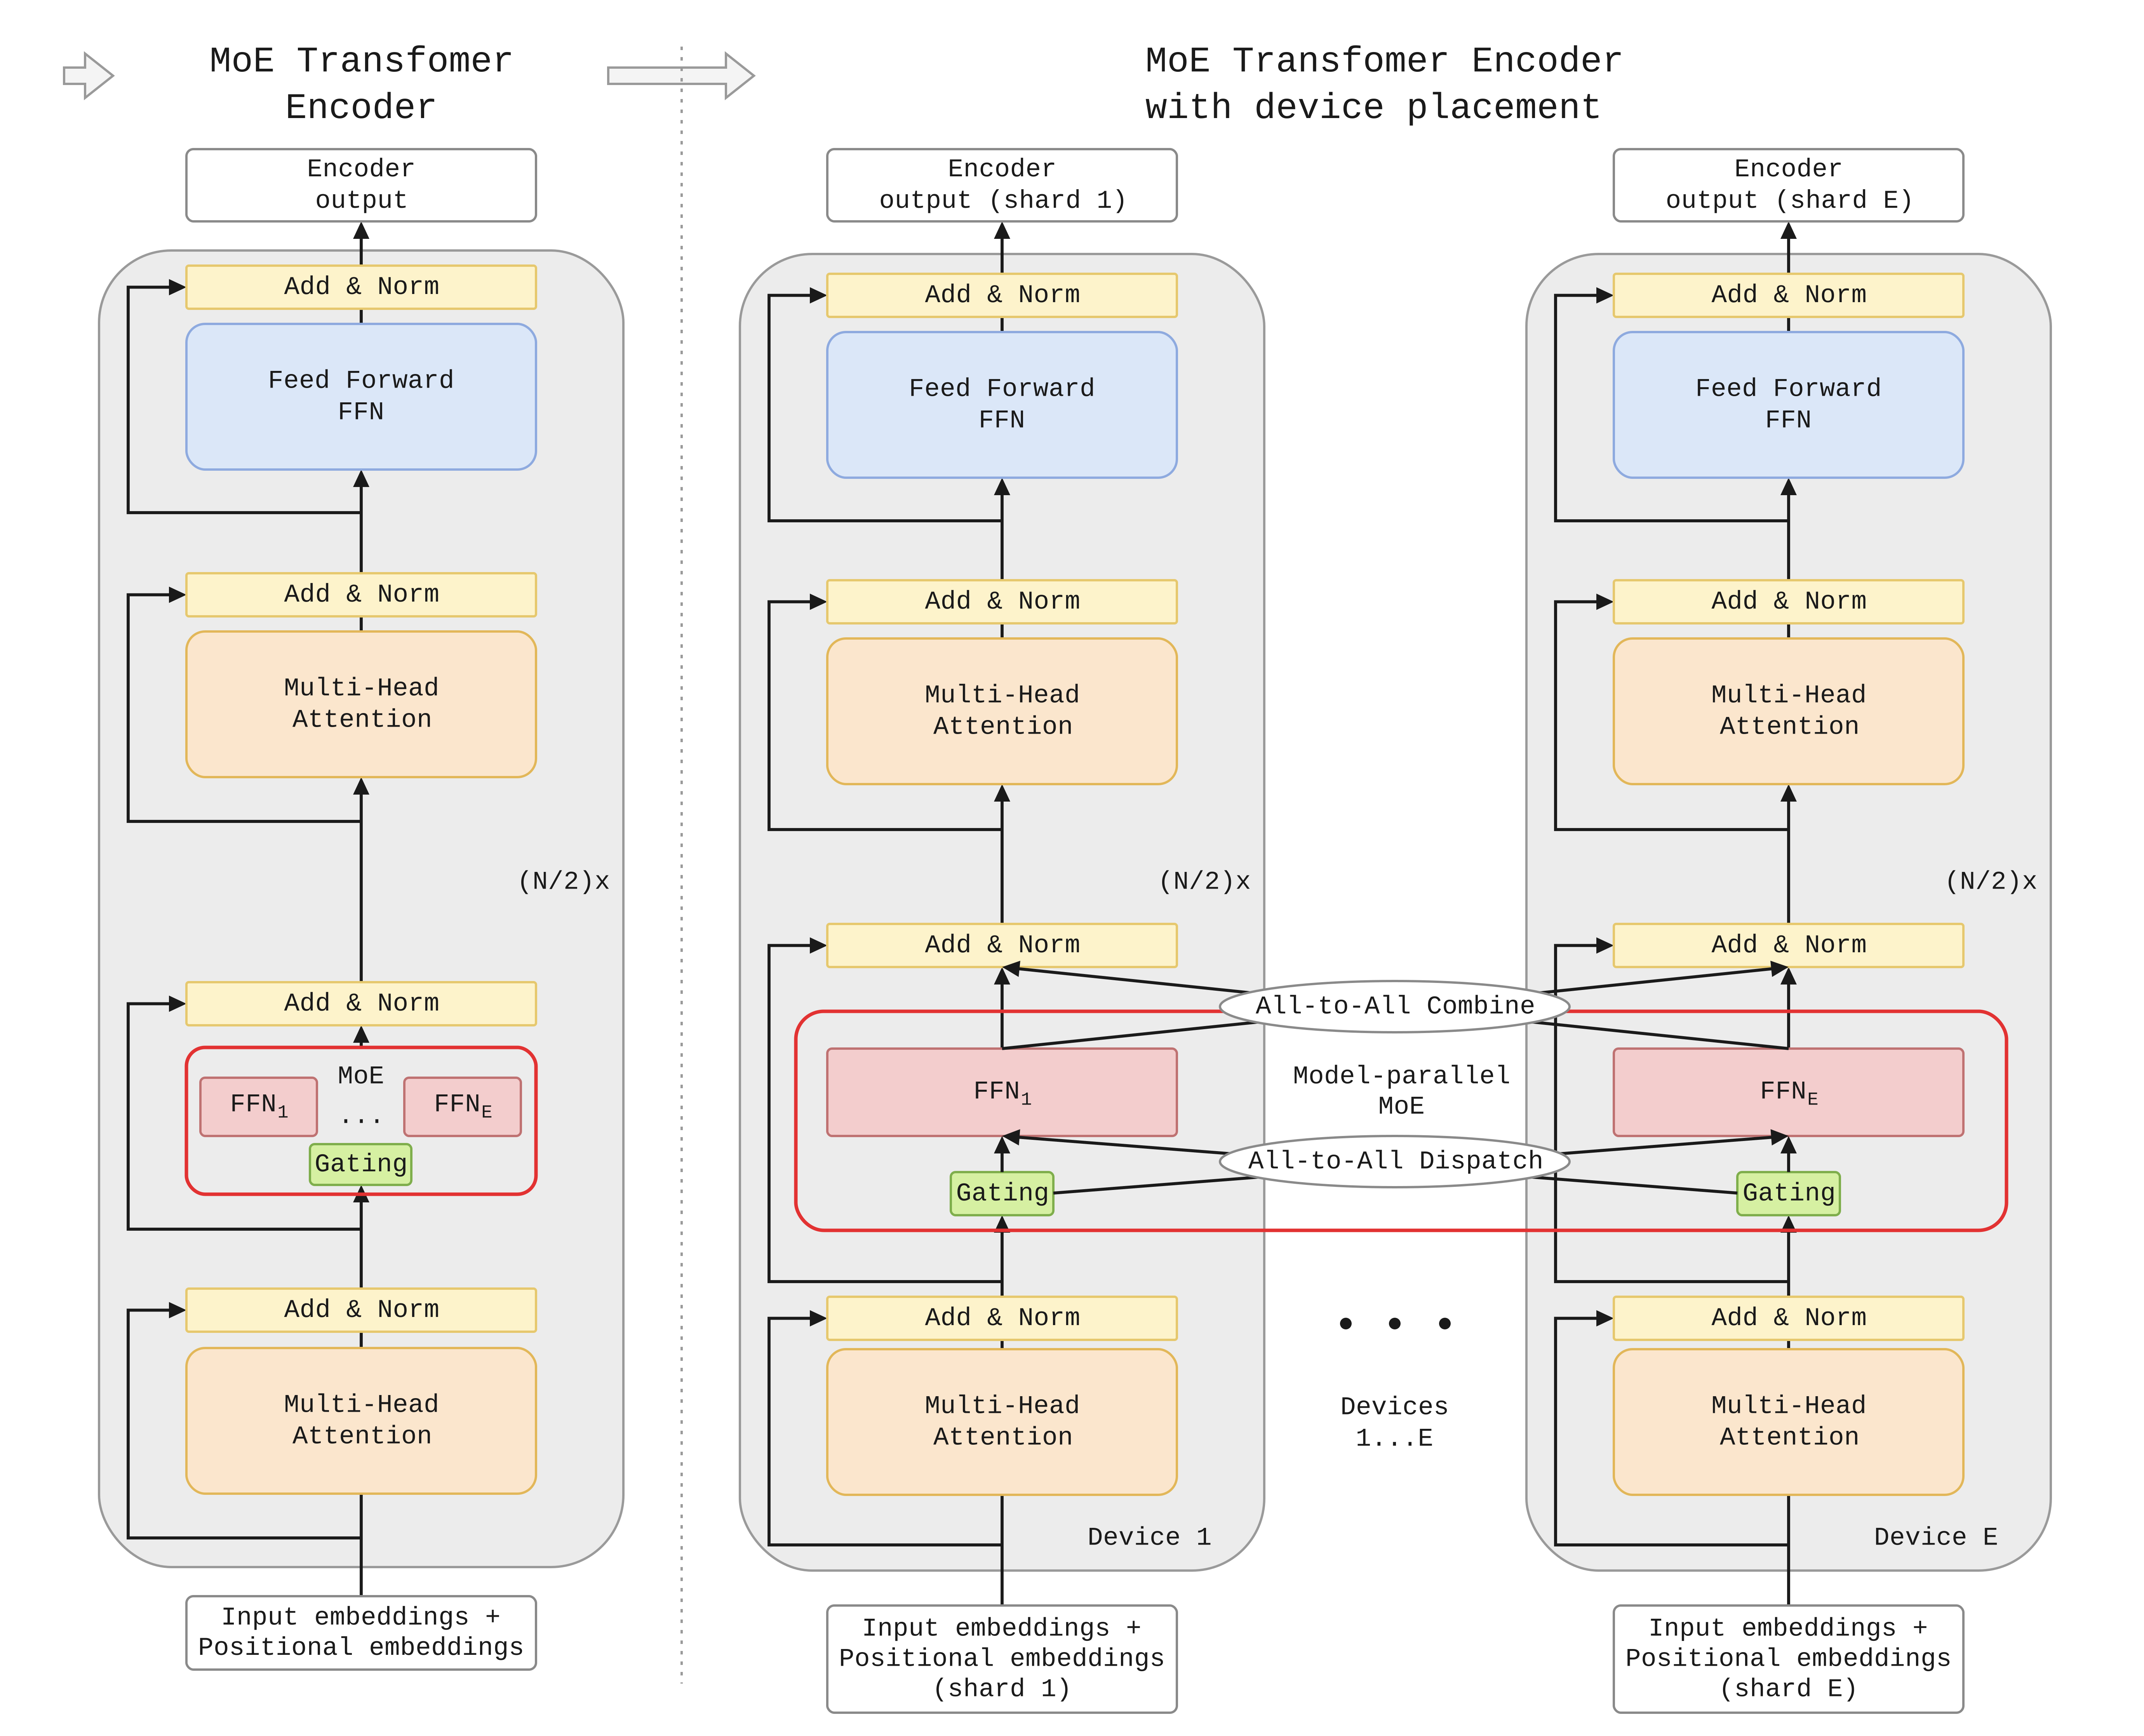
\includegraphics[width=1\linewidth]{moe_encoder.png}
\end{figure}

Putting it together to get full linear scaling for memory.

\subsubsection*{Why EP?}

EP is \textit{roughly} like TP in behavior for MLPs - high bandwidth, reduces activation.

\begin{figure}[H]
    \centering
    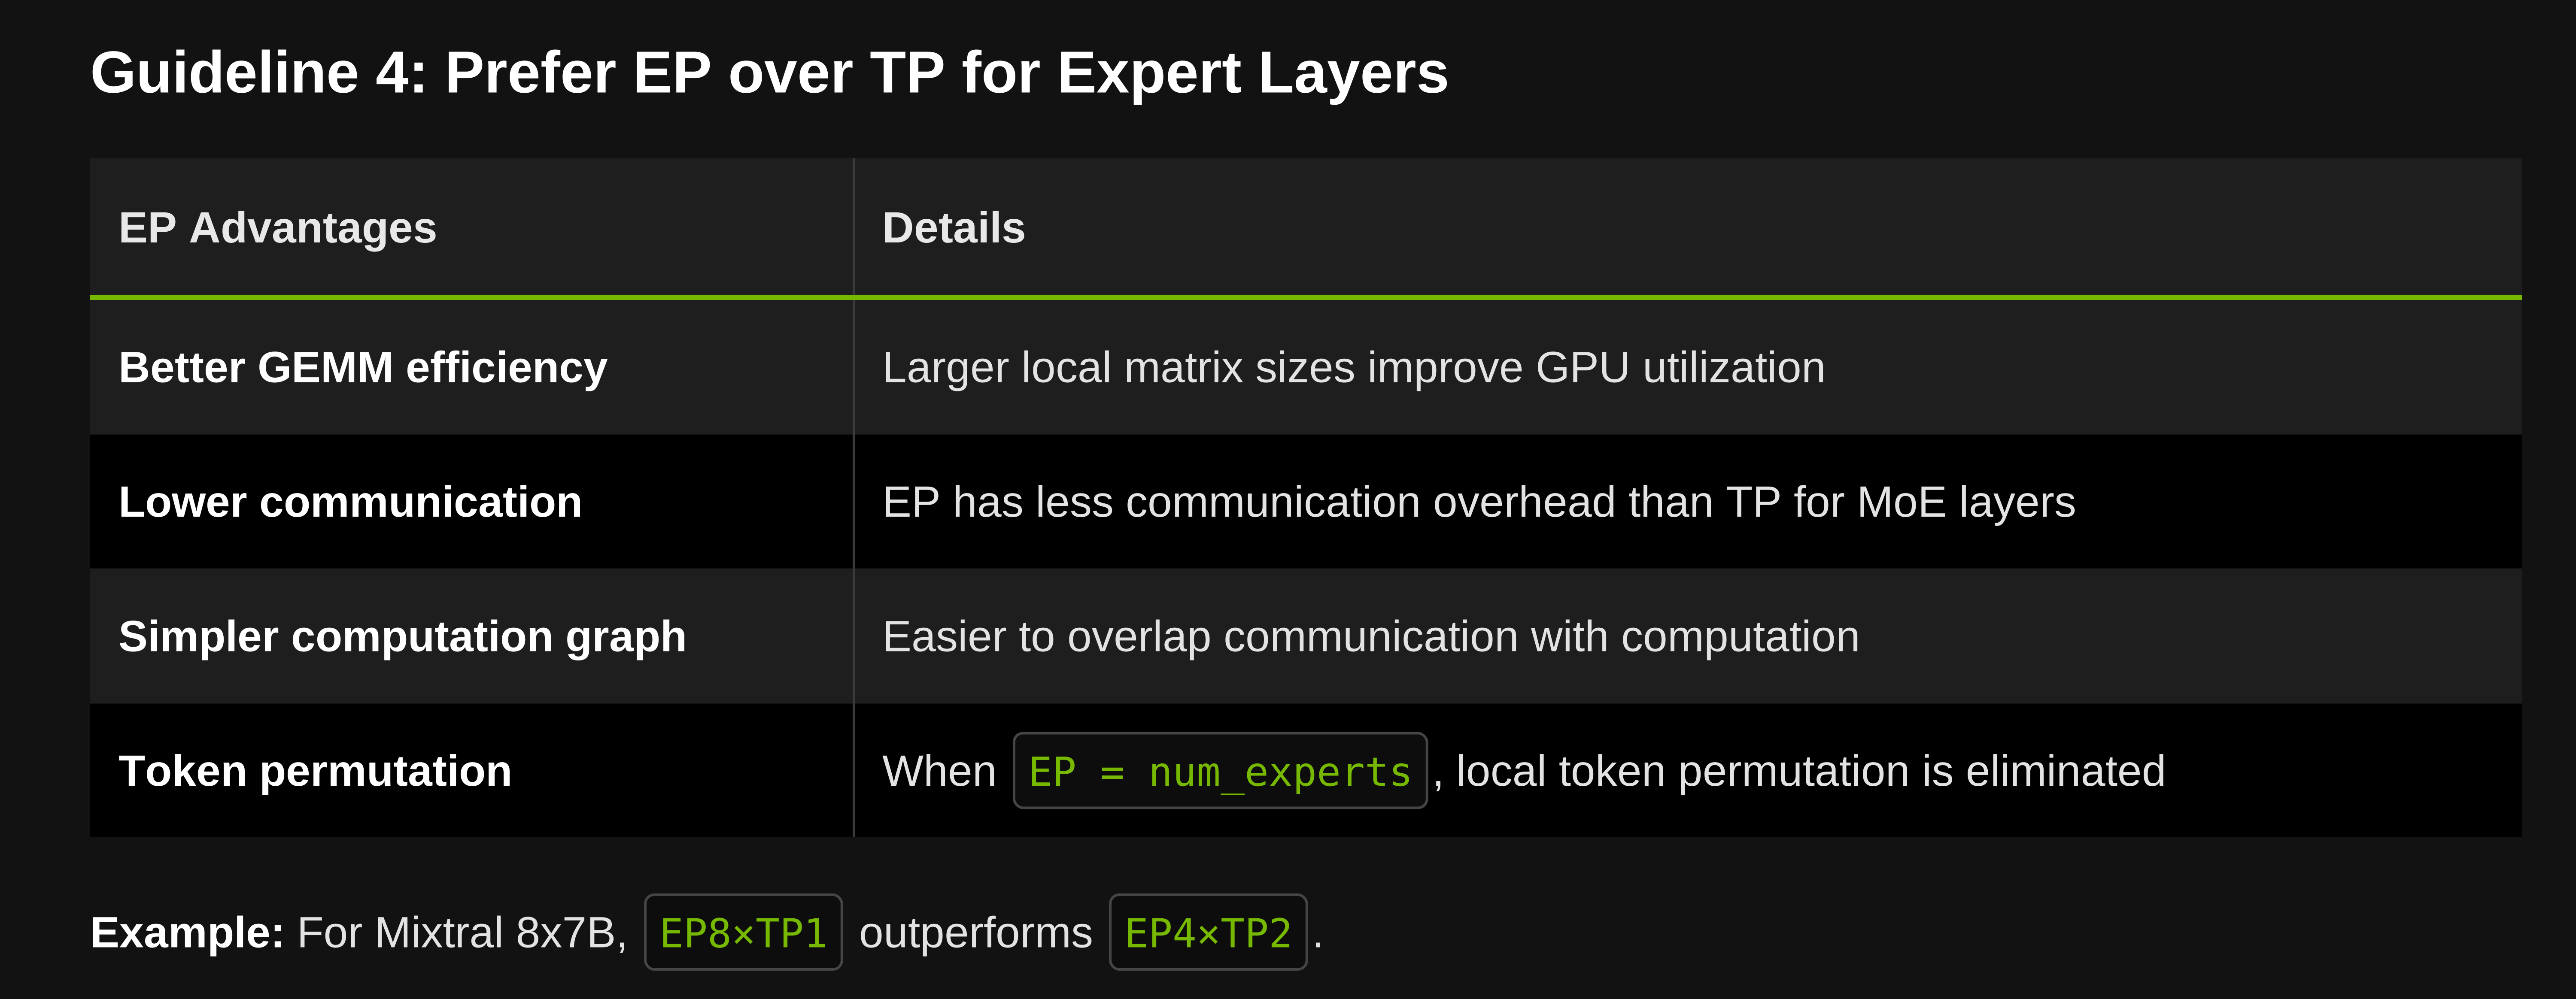
\includegraphics[width=1\linewidth]{ep_vs_tp_table.png}
\end{figure}

But, splitting matmuls can reduce efficiency verse routing activations.

\subsection*{Parallelism Complexity}

Naively - we can compose EP and all other strategies .. \textbf{but there are important notes} .. DP usually shares replicas with EP splits (so EP \(<\) DP).

\subsubsection*{Decoupling attention / expert parallelism}

This can lead to some imbalance between attention and MLPs for parallelism:

\begin{itemize}
    \item High TP - useful for attention parallelization (since we can't use EP).
    \item Low TP - useful for MLP parallelization (we'd rather EP than TP).
\end{itemize}

\textbf{Context parallel / ring attention} (split activations across GPUs in a long sequence)

\begin{figure}[hpbt]
    \centering
    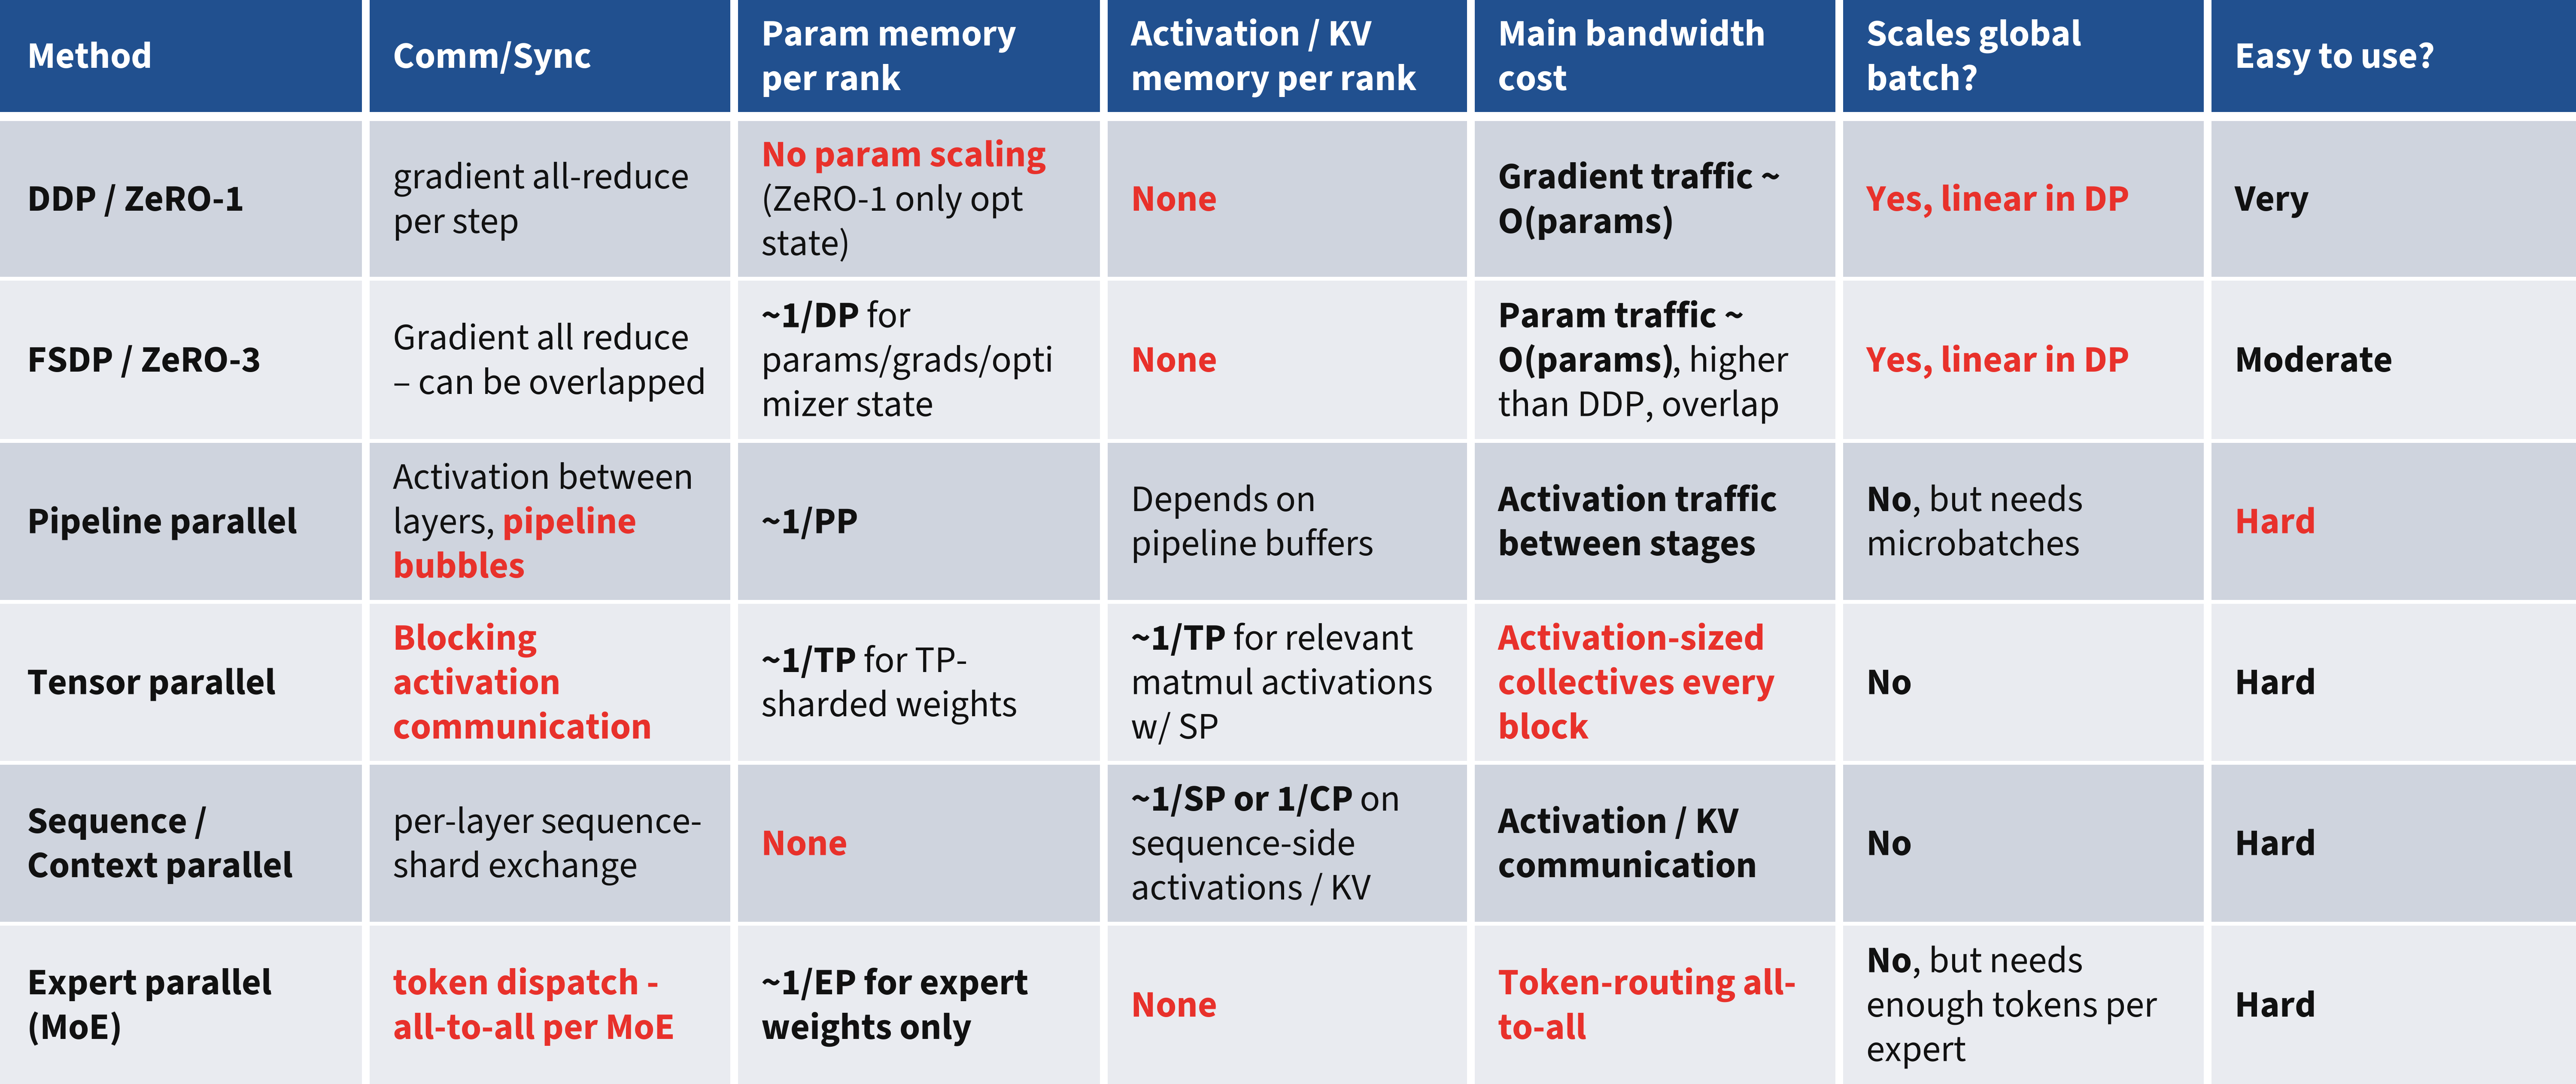
\includegraphics[width=0.91\linewidth]{parallelism_comparison.png}
\end{figure}

\subsubsection*{3D (4D) complexity - putting it all together}

\begin{center}
    Simple rules of thumb from the literature.
\end{center}

\begin{enumerate}
    \item Until your model fits in memory ..
    \begin{itemize}
        \item tensor / expert parallel up to GPUs / machine
        \item pipeline parallel across machines
        \item (or use Zero-3, depending on BW)
    \end{itemize}
    \item Then until you run out of GPUs ..
    \begin{itemize}
        \item scale the rest of the way with data parallel
        \item if your batch size is small .. gradient accumulate to trade higher batch sizes for better communication efficiency 
    \end{itemize}
\end{enumerate}

\end{document}
